\documentclass[iop,numberedappendix,apj]{emulateapj}

\usepackage{epsfig}
\usepackage{amsmath}
\usepackage{rotating}
\usepackage{natbib}
%\usepackage{lscape}
\usepackage{enumerate}
\usepackage{multirow}
\usepackage{array}
\usepackage{appendix}
\usepackage{comment}
\usepackage{color,xcolor}
\usepackage{url}
\usepackage{hyperref}
\hypersetup{colorlinks,linkcolor={blue!50!black},citecolor={blue!50!black},urlcolor={blue!50!black}}
%\usepackage[dvipdfmx]{color}
%\usepackage[dvipdfmx]{graphicx}

\bibliographystyle{apj}

\def\memoYF#1{\color{red}$[${\bf #1}$]$ \color{black}}

\def\memoDS#1{\color{blue}$[${\bf #1}$]$ \color{black}}

\def\memoNZ#1{\color{green}$[${\bf #1}$]$ \color{black}}

\definecolor{DarkGreen}{rgb}{0.0, 0.6, 0.0}
\def\memoTM#1{\color{DarkGreen}$[${\bf #1}$]$ \color{black}}

\def\plotonesc#1{\centering \leavevmode
\includegraphics[clip=, width=1.70\columnwidth]{#1}}
\def\plotoneh#1{\centering \leavevmode
\includegraphics[clip=, width=.95\columnwidth]{#1}}
\def\plotone#1{\centering \leavevmode
\includegraphics[clip=, width=.85\columnwidth]{#1}}
\def\plotoneShrinkSmall#1{\centering \leavevmode
\includegraphics[clip=, width=.49\columnwidth]{#1}}
\def\plotoneShrinkMed#1{\centering \leavevmode
\includegraphics[clip=, width=.55\columnwidth]{#1}}
\def\plotoneShrinkBig#1{\centering \leavevmode
\includegraphics[clip=, width=.65\columnwidth]{#1}}
\def\plottwo#1#2{\centering \leavevmode
\includegraphics[width=.45\columnwidth]{#1} \hfil
\includegraphics[width=.45\columnwidth]{#2}}
\def\plottwob#1#2{\centering \leavevmode
\includegraphics[width=.49\columnwidth]{#1} \hfil
\includegraphics[width=.49\columnwidth]{#2}}
\def\plottwor#1#2{\centering \leavevmode
\includegraphics[width=.55\columnwidth,angle=90]{#1} \hfil
\includegraphics[width=.55\columnwidth,angle=90]{#2}}
\def\plotthree#1#2#3{\centering \leavevmode
\includegraphics[width=.3\columnwidth]{#1} \hfil
\includegraphics[width=.3\columnwidth]{#2} \hfil
\includegraphics[width=.3\columnwidth]{#3}}

\newcommand{\cN}[1]{\mathcal{N}}
\newcommand{\pn}[1]{\mbox{$(#1)$}}
\newcommand{\spa}{\mbox{ }}
\def\gsim{\;\rlap{\lower 2.5pt
 \hbox{$\sim$}}\raise 1.5pt\hbox{$>$}\;}
\def\lsim{\;\rlap{\lower 2.5pt
   \hbox{$\sim$}}\raise 1.5pt\hbox{$<$}\;}

\newcommand{\Tcmb}{\mbox{$T_{\mbox{\tiny CMB}}$}}
\newcommand{\Tsky}{\mbox{$T_{\mbox{\tiny sky}}$}}
\newcommand{\Tsys}{\mbox{$T_{\mbox{\tiny sys}}$}}
\newcommand{\Trx}{\mbox{$T_{\mbox{\tiny rx}}$}}
\newcommand{\sigRMS}{\mbox{$\sigma_{\mbox{\tiny RMS}}$}}


% set formatting properties
\setlength{\textwidth}{6.5in}
\setlength{\textheight}{8.8in}
\setlength{\hoffset}{0.0in}
\setlength{\voffset}{-0.4in}
%\setlength{\voffset}{0.3in}
\parindent 0.2in
\parskip 0.1in



%%%%%%%%%%%%%%%%%%%%%%%%%%%%%%%%%%%%%%%%%%%%%%%%%
% THE DOCUMENT BEGINS HERE                      %
%%%%%%%%%%%%%%%%%%%%%%%%%%%%%%%%%%%%%%%%%%%%%%%%%

\slugcomment{Submitted to ApJ, XX September 2015}

\begin{document}

%%% Begin front material
%\twocolumn[%%% Begin front material

\title{Radio Emission from Red-Giant Hot Jupiters}

\author{
%
Yuka Fujii\altaffilmark{1} 
%
David S. Spiegel\altaffilmark{2,3,4}
%
Tony Mroczkowski\altaffilmark{5,6}
%
Jason Nordhaus\altaffilmark{7,8}\\
%
Neil T. Zimmerman\altaffilmark{9}
%
Aaron Parsons\altaffilmark{10}
%
Nikku Madhusudhan\altaffilmark{11}
%
Mehrdad Mirbabayi\altaffilmark{13}
}

\affil{$^1$Earth-Life Science Institute, Tokyo Institute of Technology, 
  Tokyo, JAPAN, 152-8550}
  
\affil{$^2$Analytics \& Algorithms, Stitch Fix,
  San Francisco, CA  94103}

\affil{$^3$Research \& Development, Sum Labs,
  New York, NY  10001}

\affil{$^4$Astrophysics Department, Institute for Advanced Study,
  Princeton, NJ 08540}

\affil{$^5$National Research Council Fellow}

\affil{$^6$Naval Research Laboratory, 4555 Overlook Ave SW, Washington, DC 20375}

\affil{$^7$Department of Science and Mathematics, National Technical Institute for the Deaf, Rochester Institute of Technology, Rochester, NY 14623}

\affil{$^8$Center for Computational Relativity and Gravitation, Rochester Institute of Technology, Rochester, NY 14623}

\affil{$^9$Space Telescope Science Institute, 3700 San Martin Drive, Baltimore, MD 21218}

\affil{$^{10}$Astronomy Department, University of California Berkeley}

\affil{$^{11}$Astronomy Department, University of Cambridge, UK}


\vspace{0.5\baselineskip}

\email{
yuka.fujii@elsi.jp
}


\begin{abstract}
%%%
When planet-hosting stars evolve off the main sequence and go through the red-giant branch (RGB), the stars become orders of magnitudes more luminous and at the same time lose mass at much higher rates than their main-sequence counterparts.
Accordingly, planetary companions around them at orbital distances of a few AU, if they exist, will be heated up to the level of canonical hot Jupiters and also subjected to a massive stellar wind.
Given that magnetized planets interacting with stellar winds emit radio waves, such ``Red-Giant Hot Jupiters'' (RGHJs) may also be candidate radio emitters.
We estimate the spectral auroral radio intensity of RGHJs based on the empirical relation with the stellar wind as well as a proposed scaling for planetary magnetic fields. 
We predict that RGHJs might be intrinsically as bright as canonical hot Jupiters, and 100 times brighter than equivalent objects around main-sequence stars, which allow us to search them in 1000 times larger volume. 
The signal from a RGHJ may be detectable at distances up to a few hundred parsecs with current/future instruments such as LOFAR and the Square Kilometer Array. 

%Red-giant hot Jupiters (RGHJs) are jovian planets orbiting red-giant-branch (RGB) or asymptotic-giant-branch (AGB) stars. 
%Red-giant hot Jupiters (RGHJs) are jovian planets orbiting red-giant-branch (RGB) or asymptotic-giant-branch (AGB) stars.
%Post-main-sequence stars lose mass at much higher rates than main-sequence stars.
%A jovian planet passing through the dense winds of its RGB or AGB host can capture stellar wind in its magnetosphere, leading to radio emission from electrons spiraling in the magnetic field.
%The cyclotron frequency of electrons from the stellar wind accreting onto the planet scales as 100~MHz~$(B/30 {\rm~Gauss})$.
%The cyclotron frequency of electrons from the stellar wind accreting onto the planet scales as 100~MHz~$(B/30 {\rm~Gauss})$.
%Counterintuitively, a plausible toy model suggests that a stronger planetary magnetic field leads to lower spectral flux density, and might therefore make objects more challenging to observe.
%Still, for a range of planetary and stellar parameters, a RGHJ might generate a radio luminosity that would be visible from kiloparsec distances.
\end{abstract}


\keywords{planets and satellites: Jupiter --- Sun: evolution ---
  planetary systems --- stars: evolution ---
  stars: AGB and post-AGB}
%]%%% End front material


%%%%%%%%%%%%%%%%%%%%%%%%%%%%%%%%%%%%%%%%%%%%%%%%%%%%%%%%%%%%%%%%%%%
\section{Introduction}
\label{sec:intro}
%%%%%%%%%%%%%%%%%%%%%%%%%%%%%%%%%%%%%%%%%%%%%%%%%%%%%%%%%%%%%%%%%%%


Planets with strong magnetic fields may generate radio and/or X-ray emission when interacting with energetic charged particles. 
It is well known that Jupiter emits radio waves from its auroral region due to the cyclotron-maser instability \citep[e.g.][]{wu1979,zarka1998}.  % due to the acceleration of the plasmas. \memoYF{?}.
Potentially, exoplanets can also generate radio emission through similar mechanisms, depending on their intrinsic magnetic fields and the density of surrounding plasmas, e.g. stellar wind particles and particles from Io-like moons. 
Observations of radio emission from Solar System planets imply an empirical relation that the radio intensity is proportional to the input solar wind flux going into each planetary magnetosphere, which is commonly referred to as the ``radiometric Bode's law'' \citep{desch+kaiser1984}. 
Extrapolating this scaling to exoplanets, radio emission from exoplanetary systems has been examined. 
\citet{farrell1999,zarka2001,lazio2004} estimated that a few of the known exoplanetary systems may have radio flux of $\sim $1 mJy level, due to the small orbital distance of the planet and/or the larger planetary mass. 
%\citet{griesmeier2004} modeled in detail the evolution of atmosphere and magnetic field of the tidally-locked close-in stars and found that 
\citet{stevens2005} gave improved estimates of the stellar mass-loss rate based on X-ray flux and re-evaluated the radio flux of known exoplanetary systems. 
\citet{griesmeier2005} took account of the high stellar activity in the early stage of the planetary system and proposed that the young system would be good candidates to search for radio emission. 
\citet{griesmeier2007a, griesmeier2007b} discussed the effects of the detailed properties of stellar wind in the proximity of the stars. They considered not only the kinetic energy of the stellar wind but also the magnetic energy of the stellar wind and coronal mass ejection (CME). 
Note that in these papers, the scaling relation of planetary magnetic fields differ from paper to paper.
In \citet{reiners2010}, the authors adopted a new scaling relation of planetary magnetic field based on \citet{christensen_et_al2009}. 
%\citet{jardine2008} modeled the reconnection between the magnetic fields of close-in planets and of the star, which would accelerate electrons and produce radio emission \memoTM{(can we say?) via cyclotron radiation}.
% I leave this out because this is not based on radiometric bode's law. 
Although observational searches for these radio signatures are underway, no clear detection has been claimed \citep{bastian2000,george2007,stroe2012,hallinan2013,murphy2015}, though there are some promising initial results \citep{lecavelier_et_al2013,sirothia2014}.

When stars less than $\sim$8~$M_\sun$ evolve off the main sequence, they evolve through the red-giant branch (RGB) and the asymptotic-giant branch (AGB) phases where their radii and luminosities increase by orders of magnitude.
Jovian planets in orbit around such stars can migrate inward or outward due to the interplay between tidal torques and mass-loss process on the post-main sequence \citep{nordhaus_et_al2010,nordhaus+spiegel2013}.  During this time, such planets can be transiently heated to hot-Jupiter temperatures ($\gtrsim$1000~K) at distances out to tens of AU, depending on the star's mass; such planets are termed ``Red Giant Hot Jupiters'' (RGHJs), though the term can refer to planets orbiting either RGB and AGB stars \citep{spiegel+madhusudhan2012}.
Such planets are also subject to interactions with a massive (but slow) stellar wind, as the mass-loss rate of evolved stars is significant, ranging from $\sim 10^{-8} M_\odot$/yr to $\sim  10^{-5} M_\odot$/yr with the highest values for AGB stars \citep[e.g.,][]{reimers1975, schild1989, vassiliadis1993, schoier2001, vanloon2005}. 
On the assumption that the radio emission is correlated with the stellar wind, planetary companions around evolved stars could also generate bright radio emission. 

Based on this speculation, \citet{ignace2010} examined radio emission from known substellar-mass companions around cool evolved stars.
They found that the low ionization fraction of the stellar wind of evolved stars suppresses their radio emission and leads to weak radio emission, probably below the detection limit. 

In this paper, we argue that the accretion of the massive stellar wind onto the planet would emit strong X-rays, thereby ionizing the hydrogen atoms around the planet.
The ionized stellar wind particles would then interact with the planetary magnetic field in the same way as Solar System planets do.
Thus, by extrapolating the ``radiometric Bode's law'', we provide more optimistic estimates for highly evolved stars compared to the previous result.
We also consider the plasma frequency cut-off of the stellar wind, which turns out to be one of the major obstacles to detect radio emission from RGHJs. 
Given that the survey of exoplanets around highly evolved stars is not complete, we do not constrain ourselves to the systems known to have sub-stellar companions.
Instead, we investigate the parameter space where we can search for radio emission and examine the possibility to detect them with current and future instruments. 

In Section \ref{s:assumptions}, we introduce the framework to obtain the frequency of radio emission and the planetary radio emission, and describe our models for the stellar wind and planetary magnetosphere.
Section \ref{s:result} presents an estimate of the spectral radio intensity of RGHJs and compares the predictions with what might be expected from canonical hot Jupiters as well as those from Jupiter-twins.
Section \ref{s:observability} gives the prospects for the signal detection with the current/future instruments. 
Estimates for the actual late-type (M type) evolved stars are also included. 
We find that the Square Kilometer Array(SKA), and perhaps the high band of the LOw Frequency ARray (LOFAR-HBA) as well, will be capable of detecting these signals within a reasonable integration time. 
%In \S5, we discuss the usefulness of radio emission in exploring Jupiter-like planets around evolved stars. 
Section \ref{s:discussion} is devoted to additional discussions, one for the usefulness of the radio emission for characterizing the system and the other for the effects of canceling magnetic field which results from the plasmas spiraling in the planetary magnetosphere.  
Finally, Section \ref{s:conc} concludes the paper with a brief summary. 

%Roughly 20\% of the more than 700 \memoYF{check!} currently known exoplanets around main-sequence stars \footnote{See online catalogs such as http://www.openexoplanetcatalogue.com/ \citep{rein2012}, http://exoplanet.eu \citep{schneider_et_al2011}, or http://exoplanets.org \citep{wright_et_al2011} for up-to-date lists.} have masses greater than half of Jupiter's, orbital radii greater than 1~AU, and will become hot Jupiters (i.e., for the present purposes, this means they will receive at least as much irradiation as the currently known hot Jupiters/Neptunes \citep{spiegel+madhusudhan2012}. 


%%%%%%%%%%%%%%%%%%%%%%%%%%%%%%%%%%%%%%%%%%%%%%%%%%%%%%%%%%%%%%%%%%%
\section{Model}
\label{s:assumptions}
%%%%%%%%%%%%%%%%%%%%%%%%%%%%%%%%%%%%%%%%%%%%%%%%%%%%%%%%%%%%%%%%%%%

Before estimating the frequency of planetary radio emission and its radio spectral intensity, we specify some ingredients. 
The property of the planetary magnetic field is described in \S\ref{ss:magneticfield}, and the stellar wind of the evolved stars is discussed in \S\ref{ss:stellarwind}.  
In \S\ref{ss:ionization}, we consider the ionization around the planets because it is a crucial factor to determine the efficiency of the planetary magnetosphere and the stellar wind. 
Then, we proceed to the framework to estimate the frequency and intensity of planetary radio emission in \S\ref{ss:model_frequency} and \S\ref{ss:model_intensity}, respectively. 



%%%%%%%%%%%%%%%%%%%%%%%%%%%%%%%%%%%%%%%%%%%%%%%%%%%%%%%%%%%%%%%%%%%
\subsection{Assumptions for Planetary Magnetic Field}
\label{ss:magneticfield}
%%%%%%%%%%%%%%%%%%%%%%%%%%%%%%%%%%%%%%%%%%%%%%%%%%%%%%%%%%%%%%%%%%%

We estimate the planetary magnetic field of general planets  
simply by scaling the Jovian magnetosphere at the surface $B_J \sim 10$ G according to the planetary mass and age, based on the predicted scaling relation described below. 
% we adopt a simple scaling relation between the magnetic field and macroscopic planetary properties. 

So far, several scaling relations for the planetary magnetic field strength  
have been proposed \citep[e.g.][]{russel1978,busse1976,stevenson1979,mizutani1992,sano1993,starchenko2002,christensen2006,christensen_et_al2009} %\memoYF{check!}
%(see \citet{griesmeier2004} or \citet{christensen2010} for the summary), 
which are summarized and compared with numerical simulations in \citet{christensen2010}. 
We employ the scaling law proposed in \citet{christensen_et_al2009}, which has already been used in \citet{reiners2010} to explore the evolution of planetary magnetic fields.
This scaling law is based on the assumption that the ohmic dissipation energy is a fraction of the available convected energy and was found to be in good agreement with the numerical experiments over a wide parameter space and with known objects from the Earth to stars: 
%\memoYF{describe in more detail}:
%%%%%%%%%% 
%\begin{equation}
%B^2 \propto \rho_c r_c^{4/3} q_c^{2/3}, \label{eq:Bscaling} 
%\end{equation}
\begin{equation}
B_{\rm dynamo} ^2 \propto f_{\rm ohm}\;\rho_{\rm dynamo}^{1/3} \;  (Fq_o)^{2/3} \label{eq:Bscaling} 
\end{equation}
%%%%%%%%%%
%where $\rho _c$ and $r_c$ are the density and the radius of the dynamo region, and $q_c$ is the internal convected energy flux in the core region. 
where $B_{\rm dynamo}$ is the mean magnetic field in the dynamo region, $f_{\rm ohm}$ is the ratio of ohmic dissipation to the total dissipation, $\rho_{\rm dynamo} $ is the mean density in the dynamo region, $F$ is an efficiency factor of order unity, and $q_o$ is the convected flux at the outer boundary of the dynamo region \citep[see][for the comprehensive description]{christensen_et_al2009}. 
Here, $f_{\rm ohm}$ and $F$ are assumed to be constant for the bodies considered in this paper. 
Dipole magnetic field strength at the planetary surface, denoted by $B$, is then scaled by
%%%%%%%%%%
\begin{equation}
B \propto B_{\rm dynamo} \left( \frac{r_{\rm dynamo}}{R_p} \right)^3.  \label{eq:Bscaling2}
\end{equation}
%%%%%%%%%%
where $r_{\rm dynamo}$ is the radius of the outer boundary of the dynamo region. 

Note that the scaling law, Equation (\ref{eq:Bscaling}), would be reasonable only for rapidly rotating objects.
Indeed, unlike canonical hot Jupiters, RGHJs are not tidal locked to their host stars, so we do not have to assume slow spin rotation rates \citep{spiegel+madhusudhan2012}.
Therefore, we implicitly assume that the RGHJs considered in this paper are rapidly rotating so that they generate planetary magnetic fields through the same mechanism as Jupiter. 


In order to evaluate $\rho _{\rm dynamo}$ and $q_o$, we need models of the internal planetary structure. 
We consider Jupiter-like gaseous planets and assume that the planetary radius is constant at $R_p = R_{p,J}$, as numerical calculations show that the radii of gaseous planets over the range of $0.1 M_{p, J} < M_p < 10M_{p, J}$ (with core mass less than 10\%) converge to $0.8 R_{p, J} < R_p < 1.2R_{p, J}$ within 1 Gyr \citep{fortney2007}. 
For the density profile, we assume a polytrope gas sphere with index $n=1$, which results in:
%%%%%%%%%% 
\begin{equation}
\rho [r] = \left( \frac{\pi M_p}{4 R_p^3} \right) \frac{\sin \left[ \pi \frac{r}{R_p} \right]}{\left( \pi \frac{r}{R_p} \right)}. \label{eq:rho_r}
\end{equation}
%%%%%%%%%%
We determine the radius of outer boundary of the dynamo region, $r_{\rm dynamo}$, by assuming that the hydrogen becomes metallic when $\rho (r)$ exceeds the critical density $\rho_{\rm crit}=0.7\,\mbox{g/cm}^3$ \citep{exoplanets2006, griesmeier2007b}.
The density of the metallic core, $\rho _{\rm dynamo}$ is obtained by averaging the density in the core. 
In the case of Jupiter, $r_{\rm dynamo, J} = 0.85 R_{\rm J}$ and $\rho_{\rm dynamo, J} = 1.899~{\rm g/cm}^3$.

The scaling of convected heat flux at the outer boundary, $q_o$, is obtained by dividing the age-dependent net-planetary luminosity by the surface area of the core region, i.e., $4\pi r_{\rm dynamo}^2$. 
The time-dependent luminosity is taken from equation (1) of \citet{burrows_et_al2001} \citep[see also][]{marley2007}. 
Ignoring the relatively weak dependence on average atmospheric Rosseland mean opacity leads to:
%%%%%%%%%%
\begin{equation}
%L \sim 1.84\times10^{-10} L_\odot \left( \frac{t}{4.5 \rm~Gyr} \right)^{-1.3} \left( \frac{M_p}{M_J} \right)^{2.64} \, 	
L \sim 6.3\times10^{23} \left( \frac{t}{4.5 \rm~Gyr} \right)^{-1.3} \left( \frac{M_p}{M_J} \right)^{2.64} \, 
\label{eq:burrowsLum}
\end{equation}
%%%%%%%%%%
Therefore, we have
%%%%%%%%%%
\begin{equation}
q_o \sim q_{o, J} \left( \frac{t}{4.5 \rm~Gyr} \right)^{-1.3} \left( \frac{M_p}{M_J} \right)^{2.64} \left( \frac{r_{\rm dynamo}}{r_{\rm dynamo\,J}} \right)^{-2}\, .
\label{eq:burrowsHeatFlux}
\end{equation}
%%%%%%%%%%

Substituting Equation~\ref{eq:burrowsHeatFlux} into Equation~\ref{eq:Bscaling2} and given that $r_{\rm dynamo} $ does not change significantly, the magnetic field is approximately:
%%%%%%%%%% 
\begin{equation}
%B   &\sim &  10~{\rm G} \left( \frac{t}{4.5~\rm{Gyr}} \right)^{-0.43} \left( \frac{M_p }{M_{p,J}} \right)^{1.38} \label{eq:scalingB} \\
B   \sim   10~{\rm G} \left( \frac{M_p }{M_{p,J}} \right)^{1.04} \left( \frac{t}{4.5~\rm{Gyr}} \right)^{-0.43} \label{eq:scalingB}
\end{equation}
%%%%%%%%%%
under this model. 

%We note that the scaling relation based on \citet{christensen_et_al2009}, or equation (\ref{eq:Bscaling}), has also been adopted in \citet{reiners2010}. While the detailed treatment of $\rho _c$ and $q_o$ are different, two estimates of planetary magnetic field strength are fairly close, as shown in \S3 below. 




%%%%%%%%%%%%%%%%%%%%%%%%%%%%%%%%%%%%%%%%%%%%%%%%%%%%%%%%%%%%%%%%%%%
\subsection{Assumptions for Stellar Wind}
\label{ss:stellarwind}
%%%%%%%%%%%%%%%%%%%%%%%%%%%%%%%%%%%%%%%%%%%%%%%%%%%%%%%%%%%%%%%%%%%

To model the radio emission from the interaction between the planetary magnetic field and the stellar wind,
we need the density and velocity of the stellar wind. 
The number density of particles in the stellar wind, $n$, can be expressed as
%%%%%%%%%% 
\begin{equation}
n = \frac{\dot M_\star}{4\pi a^2 m_p v_{\rm sw}}
\label{eq:n}
\end{equation}
%%%%%%%%%% 
where $\dot M_\star$ is the stellar mass loss rate, $a$ is the orbital distance from the star and $m_p$ is proton mass, and $v_{\rm sw}$ is the velocity of the stellar wind. For the solar wind, $\dot M_\odot \sim 2\times 10^{-14} M_{\odot}$/yr and $v_{\rm sw} \sim 400 {\rm km/s}$ \citep[e.g.,][]{hundhausen1997}. 

The mass loss rate of red giants is typically $\dot M_\star \sim 10^{-8}-10^{-7} M_{\odot}$/yr \citep{reimers1975}, and the rate can be as high as $10^{-5} M_\odot{\rm /yr}$ during the AGB phase \citep{schild1989, vassiliadis1993, schoier2001, vanloon2005}.
Therefore, we have
%%%%%%%%%% 
\begin{equation}
\frac{\dot M_\star}{\dot M_{\odot}} \sim 10^6 - 10^9 \, . \label{eq:scale_Mdot}
\end{equation}
%%%%%%%%%% 


On the other hand, the stellar wind velocity, $v_{\rm sw}$, becomes smaller as the star evolves. The wind velocity is typically the escape velocity at the distance of the several stellar radius \citep{suzuki2007}, i.e., $\sim \sqrt{2GM_{\star}/R'_{\star}}$ where $R'_{\star} \sim (4-5) R_{\star }$. 
For a planet with radius $R_{\star }=100~R_{\odot }$, this results in $v_{\rm sw}\sim 30~{\rm km/s}$. 
Therefore, a Solar-mass red giant with radius $R_{\star}=100R_{\odot}$ encounters at least 10 times as slow stellar wind as that at the Sun, $v_{\odot}$. 

Based on equations (\ref{eq:scale_Mdot}), the number density of the stellar wind (equation (\ref{eq:n})) are normalized as follows:
%%%%%%%%%% 
\begin{eqnarray}
n &=& 1.8 \times 10^6 \; {\rm cm^{-3}} \times \left( \frac{a}{5 \; {\rm AU}} \right)^{-2} \notag \\
&&\times \left( \frac{\dot M_\star}{10^{-8} M_{\odot }{\rm /yr}} \right) \left( \frac{v_{\rm sw}}{30~\mbox{km/s}} \right)^{-1}. \label{eq:n_normalized}
\end{eqnarray}
%%%%%%%%%% 

The contributions for the velocity term in equation (\ref{eq:Pinp_kin}), which should be the relative velocity between the planet and the solar wind, are given by the stellar wind velocity, the infall velocity (i.e., acceleration by planetary gravity), and the planetary orbital velocity. 
While $v_{\rm sw}$ is $\sim 30~{\rm km/s}$, the infall velocity at the planetary to be added is $\sim 10-25~{\rm km/s}$, depending on the planetary mass (ranging from $1 M_{\rm J}-10 M_{\rm J}$), and the orbital velocity is $10-30~{\rm km/s}$ depending on the orbital distance (ranging from $1-5~{\rm AU}$). 
Here, we simply consider
%%%%%%%%%% 
\begin{equation}
\frac{v}{v_{\odot}} \sim 10^{-1} \, . \label{eq:scale_v}
\end{equation}
%%%%%%%%%%
as a fiducial values for the normalization. 
%where $v_{\odot} \sim 4.0 \times 10^2 $ km/sec. 



%%%%%%%%%%%%%%%%%%%%%%%%%%%%%%%%%%%%%%%%%%%%%%%%%%%%%%%%%%%%%%%%%%%
\subsection{Ionization around the planet}
\label{ss:ionization}
%%%%%%%%%%%%%%%%%%%%%%%%%%%%%%%%%%%%%%%%%%%%%%%%%%%%%%%%%%%%%%%%%%%

As discussed in \citet{ignace2010}, as the stars evolve, the ionization fraction of the stellar wind are lowered down to order of $\sim 10^{-3}$ \citep{drake1987}. Since only charged particles interact with planetary magnetic field, this suggests the inefficient interaction with planetary magnetosphere and hence low input energy for radio emission. 
However, at this stage, the velocity of stellar wind becomes slower than the escape velocity of planetary companion and hence the stellar wind particles are expected to accrete onto the planets. 
\citet{spiegel+madhusudhan2012} computed the accretion luminosity $L_{\rm acc}$ and the temperature $T_{\rm acc}$ as follows: 
%%%%%%%%%
\begin{eqnarray}
L_{\rm acc} \sim &&  10^{28} \; {\rm erg\;s}^{-1} \left( \frac{\dot M_*}{10^{-8} M_{\odot }/{\rm yr}} \right)  \notag \\
&& \times \left( \frac{M_p}{10 M_J} \right)^3 \left( \frac{M_*}{M_{\odot }} \right). \\
%
T_{\rm acc} \sim && 2 \times 10^6 ~\mbox{K} \left( \frac{M_p}{10 M_J} \right) \\
\sim && 2 \times 10^5 ~\mbox{K} \left( \frac{M_p}{M_J} \right). \label{eq:Tacc}
\end{eqnarray}
%%%%%%%%%
The accretion onto planets, therefore, leads to emission of UV/X-ray radiation 
whose characteristic energy $\sim k_B T_{\rm acc} $ exceeds the ionization energy of Hydrogen, $E_{\rm Rydberg} = 13.6$~eV, or $\lambda = 91.2\rm~nm$. 

Let us consider the ionization profile around the planet. 
We suppose a state where the ionization and recombination rates are in equilibrium. 
Denoting the ionization fraction by $x$, the equilibrium state at a distance $r$ from the planet may be approximately represented by 
%%%%%%%%%
\begin{equation}
\frac{\dot N_X}{ 4 \pi r^2 } e^{- \tau } n ( 1-x ) \sigma _H [E_{\rm photon}] = (n x )^2 \beta [T_e] \label{eq:equilibrium} 
\end{equation}
%%%%%%%%%
\begin{equation}
\tau = \int _{R_J}^r n(1-x) \sigma_H dr 
\end{equation}
%%%%%%%%%
where $\dot N_X$ is the source rate of the photons that can ionize the hydrogen, 
$\sigma _H$ is the cross section of H atoms for X-ray \citep{verner1996}: 
%%%%%%%%%
\begin{equation}
\sigma _H [E_{\rm photon}] \sim 6.3 \times 10^{-18} \;{\rm cm}^2 \cdot \left( \frac{E_{\rm photon}}{E_{\rm Rydberg}} \right)^{-3} \label{eq:sigma_H}
\end{equation}
%%%%%%%%%
where $E_{\rm photon}$ is the energy per photon, 
and $\beta [T_e]$ is the ``class B'' recombination coefficient which is 
$ \beta \sim 2.6 \times 10^{-13}\;{\rm cm^3/sec} $ \citep{pequignot1991} 
at electron temperature of stellar wind of evolved stars, $T_e \sim 10^4 $K \citep{suzuki2007}. 


The source rate is obtained by counting the number of photons whose energy exceeds the ionization energy of Hydrogen ($E_{\rm Rydberg} = 13.6$~eV, %where Ry is the Rydberg constant, 
or $\lambda = 91.2\rm~nm$), which is approximately given by dividing the X-ray accretion luminosity by the characteristic photon energy produced:
%%%%%%%%%
\begin{equation}
\dot{N}_X \sim \frac{L_{\rm acc}}{k_B T_{\rm acc}} \, ,
\end{equation}
%%%%%%%%%
where $k_B$ is Boltzmann's constant.
As a result, 
%%%%%%%%%
\begin{eqnarray}
\dot{N}_X \sim  
  \left\{
    \begin{array}{ll}
      2 \times 10^{35} \;  {\rm sec^{-1}} & \;\;\;(M_p = M_J) \\
      3 \times 10^{37} \; {\rm sec^{-1}} & \;\;\;(M_p = 10 M_J)
    \end{array}. 
  \right.
\end{eqnarray}
%%%%%%%%%

For the accretion onto large planets, however, the characteristic photon energy is so high (equation (\ref{eq:Tacc})) that the released energetic electrons may also ionize other atoms in the vicinity.
The cross section\footnote{This is close to the geometric cross section of the Bohr radius.} of hydrogen for electrons is $\sim 4\times 10^{-17} {\rm cm}^2$ (\citep{fite1958}), which implies a mean free path for ionized electrons of $\sim$2$R_J$ in the surrounding medium.
As a result, nearly 2/3 of released energetic electrons will ionize a hydrogen atom within $\sim$2$R_J$, and more than 99\% will ionize a hydrogen atom within $\sim$10$R_J$.

In principle, photons with energy $E_{\rm photon}$ have potential to ionize $E_{\rm photon}/E_{\rm Rydberg}$ times.
To take this into account, we consider two limiting possibilities:
After an ionizing collision, the energy can (\emph{i}) be split evenly between the two electrons, or it can (\emph{ii}) go entirely into the kinetic energy of one electron and not at all into that of the other (of course, any split in between these extremes is possible, too).
Note that conservation of momentum and energy imply that the proton will not acquire a significant fraction of the energy of the collision.\footnote{Were it otherwise, we'd have to take into account what fraction of a rubber ball's kinetic energy is imparted to the kinetic energy of the Earth when bouncing a ball.}  

Scenario (\emph{i}) implies a cascade where an electron with energy $E_{\rm in}$ ionizes an atom producing two electrons (an ionizing electron plus the released electron) with energy $ ( E_{\rm in} - E_{\rm Rydberg} ) /2 $ for each.
For example, in an idealized case with $M_p = 10 M_{\rm J}$, $k_B T_{\rm acc} \sim 172\,{\rm eV} \sim 12 \, E_{\rm Rydberg}$, a photoionization could produce an electron with energy of $(12-1) = 11 E_{\rm Rydberg} $, then a second ionization by that electron would produce two photons with energy of $(11-1)/2 = 5 E_{\rm Rydberg}$, and the third ionization by these two photons would produce four photons with energy of $(5-1)/2 = 2 E_{\rm Rydberg}$, etc.
The cascade can proceed to the fourth order at the maximum.

Under scenario (\emph{ii}), the cascade proceeds with the initial $E_{\rm in}$ electron leading to an electron with kinetic energy $E_{\rm in} - E_{\rm Rydberg}$ and another electron with 0 kinetic energy.
Clearly, this cascade can produce a maximum total of $E_{\rm in} / E_{\rm Rydberg}$ free electrons.

In reality, not all released electrons may be able to proceed the next ionization.
If $\xi$ represents the fraction of released electrons that proceed to the next ionization, then the number of ionized atoms $N_i$ released through this cascade (\emph{i}), is
%%%%%%%%%
\begin{eqnarray}
  \nonumber N_i & = & (1-\xi) + 2\xi (1-\xi) + 4 \xi^2 (1-\xi) + 8 \xi^3 \\
  \label{eq:N_i1} & = & 1 + \xi + 2 \xi^2 + 4 \xi ^3 \, .
\end{eqnarray}
%%%%%%%%%
%With $\xi = 0.8 $, this gives $N_i \sim 5$.  \memoDS{Why 0.8?}
Alternatively, cascade (\emph{ii}) leads to
%%%%%%%%%
\begin{eqnarray}
  \nonumber N_i & = & \frac{1 - \xi^\nu}{1 - \xi} \\
  \label{eq:N_i2}  & = & 1 + \xi + \xi^2 + \cdots + \xi^{\nu - 1} \, ,
\end{eqnarray}
%%%%%%%%%
where $\nu \equiv E_{\rm in} / E_{\rm Rydberg}$ is the maximum number of ionizations for the given initial electron energy.
This limit leads to a value for $N_i$ that is not dramatically different from that of limit (\emph{ii}).
In Appendix \ref{sec:AppendixB}, we estimate the Bhabha(/M{\o}ller) scattering cross section and show that cascade (\emph{ii}) is probably more realistic.

Ultimately, $\dot{N}_X $ in equation (\ref{eq:equilibrium}) is replaced by 
%%%%%%%%%
\begin{equation}
\dot{N}_X \rightarrow N_i \dot{N}_X \, .
\end{equation}
%%%%%%%%%
For a $10 M_J$ planet, $N_i$ is probably approximately in the range 5---10.

The ionization fraction $x$ as a solution of equation (\ref{eq:equilibrium}) is shown in Figure \ref{fig:ionizationfraction}. 
%\memoDS{We should write the expression ... it's just the quadratic formula, but it would be useful to write.}
When, $\tau \sim n \sigma _H r$ is much smaller than unity and thus $e^{-\tau }$ term can be ignored (that is the case for $M_p = 10 M_J$),  the solution is simply
%%%%%%%%%
\begin{eqnarray}
x[r] &=& \frac{-1 + \sqrt{1+4C[r]}}{2C[r]} \\
C[r] &\equiv &   \frac{4 \pi n \beta [T_e] r^2}{\dot{N} \sigma_H[E_{\rm photon}]}  \end{eqnarray}
%%%%%%%%%
The solid lines show the ionization fraction of $\xi=0$ (no additional ionization by electrons) and dashed lines show that of $\xi=0.5$. In the figure, the vertical lines show the magnetic stand-off points obtained by equation (\ref{eq:stand-off-radius}) below. 
While the photon rate is large for larger planets, the strong dependence of cross section on the photon energy (equation (\ref{eq:sigma_H})) leads to the decrease in the radius of ionized region. 
Nevertheless, still, substantial amount of ionized plasmas are expected around the magnetic stand-off radius. 

The extent of ionized region can also be roughly estimated by Stromgren radius of the accretion disk \citep{stromgren1939}: 
%%%%%%%%%
\begin{equation}
r_{\rm stromgren} = \left( \frac{3}{4\pi} \frac{\dot N_X}{n^2 \beta } \right)^{1/3}
\end{equation}
%%%%%%%%%
which gives
%%%%%%%%%
\begin{eqnarray}
r_{\rm stromgren} \sim  
  \left\{
    \begin{array}{ll}
      67 ~R_J & \;\;\;(M_p = M_J) \\
      310 ~R_J & \;\;\;(M_p = 10 M_J)
    \end{array}
  \right. \label{eq:stromgren}
\end{eqnarray}
%%%%%%%%%
for a planet around a red giants at 5~AU. 
The Stromgren radius for $1M_J $ and for $10M_J$ are also indicated in Figure \ref{fig:ionizationfraction}. Note, however, that unlike the frequently-demonstrated photoionization problem around O/B-type stars, in the situation of our interest, the Stromgren radius is not a sharp edge of ionization anymore, due to smaller source rate and smaller cross section (in this case parameter ``a'' in equation (13) of \citet{stromgren1939} is not small). 
The Stromgren radii are indicated by vertical arrows in Figure \ref{fig:ionizationfraction}. 


%%%%%%%%%%%%%%%%%%%%%%%%%%%%%%%%%%%
\begin{figure}[htbp]
   \plotoneh{ionizationfraction.pdf}
   \caption{Profile of ionization fraction due to X-ray from the planetary accretion disk, measured from the surface of the planet. Solid lines show the solutions without the correction for the secondary ionization by ionized electrons, while the dashed lines show the solutions which take the correction into account with efficiency factor $\xi=0.8$. The vertical arrows show the Stromgren radius estimated simply  by equation (\ref{eq:stromgren}). The dotted vertical lines indicate the location of the magnetic stand-off radii, $r_{\rm mag}$,  obtained by equation (\ref{eq:stand-off-radius}) below. }
   %\memoDS{This looks great.  Might be good to also show the locations of the magnetic standoff point and the ``stromgren sphere radius'' on this figure (say, with vertical dashed and dotted lines?), and to move the legend to the lower left corner? {\tt plt.legend(loc=3)}}
  \label{fig:ionizationfraction}
\end{figure}
%%%%%%%%%%%%%%%%%%%%%%%%%%%%%%%%%%% 

We therefore expect for the X-ray emission from the accretion disk to ionize the stellar wind.
This implies that the stellar wind particles represented by (equation~(\ref{eq:n})) are fully ionized plasmas like Solar wind, and that the stellar wind can interact with the planetary magnetic fields in a rather similar way to the case of Solar System planets.



%\citet{drake1983}
%\citet{}
%\color{black}

%The temperature of stellar wind of RGs is expected to be 2 orders of magnitude lower than their main sequence counterparts, mainly because the sound speed of hot corona exceeds the escape speed, i.e., hot corona cannot be confined in the stellar atmosphere \citep{suzuki2008}. 
%\begin{equation}
%\frac{T}{T_{\odot}} \sim 10^{-2}
%\end{equation}
%where $T_{\odot } \sim 10^6$ K. 

%%%%%%%%%%%%%%%%%%%%%%%%%%%%%%%%%%%%%%%%%%%%%%%%%%%%%%%%%%%%%%%%%%%
\subsection{Frequency of Radio Emission}
\label{ss:model_frequency}
%%%%%%%%%%%%%%%%%%%%%%%%%%%%%%%%%%%%%%%%%%%%%%%%%%%%%%%%%%%%%%%%%%%

Planetary auroral radio wave are emitted at the local cyclotron frequency along the motion of the plasmas.
The upper limit is around the cyclotron frequency of the planetary surface magnetic field, $\nu_{\rm cyc}$: 
%%%%%%%%%% 
\begin{equation}
\nu_{\rm cyc} = \frac{eB}{2\pi m_e c} \approx 28 {\rm~MHz} \left( \frac{B}{10 \rm~G} \right) \label{eq:fcyc}
\end{equation}
%%%%%%%%%%
where $e$ and $m_e$ are the charge and mass of the electron, respectively.

Radio emission from the planet is observable from ground only when the frequencies of the radio emission are larger than the plasma frequency of Earth's ionosphere $\nu_{\rm plasma}^\oplus$ and the maximum plasma frequency along the line of sight $\nu_{\rm plasma}^{\rm los}$.
The plasma frequency may be expressed as
\begin{eqnarray}
\nu_{\rm plasma} & = & \sqrt{\frac{n_e e^2}{\pi m_e}} \\
 & = & 8979 {\rm~Hz} \times \left( \frac{n_e}{\rm cm^{-3}} \right)^{1/2} \, .
\label{eq:fplasma}
\end{eqnarray}
In the Earth's ionosphere, the electron number density is less than $10^6$~cm$^{-3}$, which implies that $\nu_{\rm plasma}^\oplus \lsim 10$~MHz.
At the favorable viewing condition, when the planet is on the near side of its star to the Earth, the maximum plasma frequency along the line of sight corresponds to that in the vicinity of the planet.
Therefore, combining Eq.~(\ref{eq:n_normalized}) and Eq.~(\ref{eq:fplasma}), we have
%%%
\begin{eqnarray}
\label{eq:fplasmalos} \nu_{\rm plasma}^{\rm los} & \sim & 
8979 {\rm~kHz} \times \left( \frac{\dot M_\star}{4 \pi a^2 m_p v} \times 1\rm~cm^3 \right)^{1/2} \\
\label{eq:fplasmalos_scaled} &=& 12 {\rm~MHz} \times \left( \frac{a}{5~\mbox{AU}}\right)^{-1} \left(\frac{v}{30~\mbox{km/s}}  \right)^{-1/2} \notag \\
 & & \times \left( \frac{\dot M_\star}{10^{-8} M_{\odot }{\rm /yr}}\right)^{1/2} \, .
\end{eqnarray}
%%%
%where in Eq.~(\ref{eq:fplasmalos_scaled}) we have taken the solar mass-loss rate $\dot M_\odot$ to be $2.0 \times 10^{-14}~M_\odot$/yr and the typical solar wind velocity $v_{\odot }$ to be 400~km/sec.

%%%%%%%%%%%%%%%%%%%%%%%%%%%%%%%%%%%%%%%%%%%%%%%%%%%%%%%%%%%%%%%%%%%
\subsection{Flux of Radio Emission}
\label{ss:model_intensity}
%%%%%%%%%%%%%%%%%%%%%%%%%%%%%%%%%%%%%%%%%%%%%%%%%%%%%%%%%%%%%%%%%%%

The auroral radio spectral flux of exoplanets observed at the Earth, $F_{\nu}$, can be expressed by:
%%%
\begin{equation}
F_{\nu} = \frac{P_{\rm radio}}{\Omega l^2 \Delta \nu}
\label{eq:Fnu}
\end{equation}
%%%
where $P_{\rm radio}$ is the energy that is deposited as radio emission of considered frequency range, $\Omega$ is the solid angle of the emission, $l$ is the distance between the target and the Earth, and $\Delta \nu$ is frequency bandwidth. 

We estimate the radio emission of exoplanets, $P_{\rm radio}$, simply by scaling the Jovian auroral radio emission, $P_{\rm radio,\,J}$, with the input energy from stellar wind, in the same manner as \citet{griesmeier2005,griesmeier2007a,griesmeier2007b}.
The scaling is based on the empirical/apparent good correlation between the radio emission intensity of Solar System planets and the input kinetic energy, $P_{\rm inp,\,k}$, or the magnetic energy of the solar wind, $P_{\rm inp,\,m}$, \citep[``radiometric Bode's law''; ][]{desch+kaiser1984}, i.e.,
%Namely, although the detail of the mechanism to generate planetary radio emission is not fully understood so far \memoYF{cite something?}, 
%observations indicate that the total radio emission, $P_{\rm radio}$ is proportional to the input kinetic energy, $P_{\rm k,\,inp}$, or the input magnetic energy, $P_{\rm m,\,inp}$ \citep[``radio Bode's law''; ][]{desch+kaiser1984}:
%%%
\begin{eqnarray}
P_{\rm radio} &\propto & P_{\rm inp} \\
P_{\rm inp,\,k} &=& n v^3 r_{\rm mag} ^2 \label{eq:Pinp_kin}, \\
P_{\rm inp,\,m} &=& v B_{\bot }^2 r_{\rm mag} ^2 \label{eq:Pinp_mag} \, ,
\end{eqnarray}
%%%
where $ B_{\bot }$ is the interstellar magnetic field perpendicular to the stellar wind flow, and $r_{\rm mag}$ is the radius of the magnetic stand-off point. 
%In the case of the Solar wind, the kinetic energy is dominant input energy over the magnetic one (the former is $\sim 400$ times larger than the latter).  
It is not clear from the observations of the Solar System planets which is the fundamental one, the correlation to the input kinetic energy, that to the magnetic energy, or both. 
In this paper, we assume that the radio emission is scaled with the input kinetic energy, i.e., $P_{\rm radio} \propto P_{\rm k,\,inp}$ and consider the possible effects of massive stellar wind. 

In the case that the correlation with input magnetic energy is fundamental, it is difficult to estimate the planetary radio emission at this point because magnetic field of evolved stars are not well constrained for highly evolved stars; most of observations only set an upper limit \citep[e.g.,][]{konstantinova2010,petit2013,tsvetkova2013,konstantinova2013,auriere2015}. 
In the case of M-type giant EK boo, surface magnetic field $\sim 0.1-10 $G has been measured; In this particular case, given the large stellar radius $R_\star \sim 210 R_{\odot }$ the magnetic moment may be about $10^3$ times larger than the Sun and thus may also increase the planetary radio emission.
However, because of the lack of universal understanding of the stellar magnetic field, we leave the magnetic model of radio emission for evolved stars for future work. 

In reality, the total power of Jovian auroral emission varies greatly over time: $1.3\times 10^{10}$ W for the average, $3.2\times 10^{10}$ W for the average of highly active time, and $4.5 \times 10^{11}$ W for the peak activity \citep{zarka_et_al2004}. 
Here we employ $P_{\rm radio,\,J}=2.1\times 10^{11}\mbox{~W}$ as a canonical value, following \citet{griesmeier2005,griesmeier2007b}. 

The radius of the magnetic stand-off point, $r_{\rm mag}$, is obtained based on the balance between the stellar wind pressure and the planetary magnetic pressure: 
%%%
\begin{equation}
m_p n v ^2 \sim \frac{B^2}{8\pi}\left( \frac{r_{\rm mag}}{R_p} \right)^{-6}  \label{eq:stand-off}
\end{equation}
%%%
The radius obtained for Jupiter from this equality is about half of the actual magnetospheric radius \citep[][]{griesmeier2005}. 
By scaling this radius with equations (\ref{eq:n}) and (\ref{eq:stand-off}), the radius of magnetosphere of planets would be estimated as:
%If the radius of magnetosphere is estimated by scaling that of Jupiter according to equations (\ref{eq:n}) and (\ref{eq:stand-off}), 
%We estimate $r_{\rm mag}$ simply by scaling Jovian magnetosphere \citep[$r_{s,\,J} \sim 84 R_J$;][]{joy2002} according to equation (\ref{eq:stand-off}), i.e., 
%%%
\begin{eqnarray}
\nonumber r_{\rm mag} 
%&\sim & R_p \left( \frac{B^2}{8\pi m_{\rm p}nv^2} \right)^{1/6}  \\
&=& r_{mag,\,J} \left( \frac{B}{10~\mbox{G}} \right)^{1/3} \left( \frac{a}{5.2\mbox{AU}} \right)^{1/3}  \\
&& \times \left( \frac{\dot M_\star}{\dot M_\odot} \right)^{-1/6}  \left( \frac{v}{v_{\odot }} \right)^{-1/6} \\
\nonumber &=& 15 \, R_J \left( \frac{B}{10~\mbox{G}} \right)^{1/3}  \left( \frac{a}{5\mbox{AU}} \right)^{1/3} \\
&& \times \left( \frac{\dot M_\star}{10^{-8} M_{\odot }{\rm /yr}} \right)^{-1/6}  \left( \frac{v}{10^{-1}v_{\odot }} \right)^{-1/6}
 \label{eq:stand-off-radius}
\end{eqnarray}
%%%

%Thus, the radio emission, $P_{\rm radio}$, or equivalently the input kinetic energy, $P_{\rm k,\,inp}$, are estimated with $n$, $v$, and $\mathcal{M}$, which should be specified by assuming the properties of the stellar wind and the planetary magnetic field. 
%In the following, we describe our assumptions for these properties. 

We assume that the solid angle of the emission, $\Omega $, is same as the Jupiter's one for all of the exoplanets.
In reality, the solid angles of auroral radio emission from  Jupiter, Saturn, and Earth are $\sim 1.6$, $\sim $6.3, and $\sim $3.5, respectively \citep{desch+kaiser1984}, which are on the same order and will not significantly affect our order-of-magnitude estimate of radio emission. 
The bandwidth, $\Delta \nu$, is assumed to be proportional to the representative frequency of the emission, which is the cyclotron frequency, following \citet{griesmeier2007b}.

%We estimate the radio brightness of RGHJs by simply scaling \memoDS{stray sentence fragment?}


%%%%%%%%%%%%%%%%%%%%%%%%%%%%%%%%%%%%%%%%%%%%%%%%%%%%%%%%%%%%%%%%%%%
\section{Results}
\label{s:result}
%%%%%%%%%%%%%%%%%%%%%%%%%%%%%%%%%%%%%%%%%%%%%%%%%%%%%%%%%%%%%%%%%%%

%%%%%%%%%%%%%%%%%%%%%%%%%%%%%%%%%%%%%%%%%%%%%%%%%%%%%%%%%%%%%%%%%%%
\subsection{Estimate of Planetary Magnetic Field and Maximum Frequency}
\label{ss:Bplanet}
%%%%%%%%%%%%%%%%%%%%%%%%%%%%%%%%%%%%%%%%%%%%%%%%%%%%%%%%%%%%%%%%%%%s

Figure \ref{fig:planetaryB_pre} shows the computed radius ($r_c$) and average density ($\rho_c$) of the dynamo region, and Figure \ref{fig:planetaryB} displays the estimates of the strength of planetary magnetic field $B$ based on the scaling relation in \S\ref{ss:magneticfield} and the corresponding cyclotron frequency ($\nu_{\rm cyc}$), as functions of planetary mass and the age. 
%Given that $\rho _c \propto M_p$  at large $M_p$ and $q_c \propto t^{-1.3} M_p^{2.64}/r_c^2$, the magnetic field is roughly:
Reasonably, the resultant values agree with \citet{reiners2010}, who adopted the same scaling law for planetary magnetic field; we show this figure just for completeness. 

%%%%%%%%%% 
%\begin{eqnarray}
%B   &\sim &  10~{\rm G} \left( \frac{t}{4.5~\rm{Gyr}} \right)^{-0.43} \left( \frac{M_p }{M_{p,J}} \right)^{1.38} \label{eq:scalingB} \\
%B   &\sim &  10~{\rm G} \left( \frac{t}{4.5~\rm{Gyr}} \right)^{-0.43} \left( \frac{M_p }{M_{p,J}} \right)^{1.04} \label{eq:scalingB} \\
%\nu_{\rm cyc} &\sim &  28~{\rm MHz} \left( \frac{t}{4.5~\rm{Gyr}} \right)^{-0.43} \left( \frac{M_p }{M_{p,J}} \right)^{1.38} \label{eq:scalingfc} 
%\nu_{\rm cyc} &\sim &  28~{\rm MHz} \left( \frac{t}{4.5~\rm{Gyr}} \right)^{-0.43} \left( \frac{M_p }{M_{p,J}} \right)^{1.04} \label{eq:scalingfc} 
%\end{eqnarray}
%%%%%%%%%%
%under this model. 
Note that the cyclotron frequency of Jovian planets typically falls between 10~MHz ($\sim $ the plasma cut-off frequency of Earth's ionosphere) and 1~GHz. 
In this regime, there are a number of current and near-future radio wave detectors including GMRT, 
LOFAR, HERA, SKA, and potential upgrades to the VLA. 



%%%%%%%%%%%%%%%%%%%%%%%%%%%%%%%%%%%
\begin{figure}[htbp]
   \plotoneh{fig1_linear.pdf}
   \caption{Radius and average density of the dynamo region as a function of planetary mass. }
  \label{fig:planetaryB_pre}
\end{figure}
%%%%%%%%%%%%%%%%%%%%%%%%%%%%%%%%%%% 

%%%%%%%%%%%%%%%%%%%%%%%%%%%%%%%%%%%
\begin{figure}[htbp]
   \plotoneh{fig2_Christensen.pdf}
   \caption{Planetary magnetic field as a function of age for different planetary mass, based on the scaling of magnetic field of \citet{christensen2010} and the evolution of luminosity of \citet{burrows_et_al2001}.} %\memoDS{Can we change density to cgs in this figure?}
  \label{fig:planetaryB}
\end{figure}
%%%%%%%%%%%%%%%%%%%%%%%%%%%%%%%%%%% 


%%%%%%%%%%%%%%%%%%%%%%%%%%%%%%%%%%%%%%%%%%%%%%%%%%%%%%%%%%%%%%%%%%%
\subsection{Estimate of Radio Intensity of RGHJs in comparison with canonical HJs}
\label{ss:brightness}
%%%%%%%%%%%%%%%%%%%%%%%%%%%%%%%%%%%%%%%%%%%%%%%%%%%%%%%%%%%%%%%%%%%

Based on the assumption that the radio emission is proportional to the input kinetic energy (equation (\ref{eq:Pinp_kin})), the scaling of the radio emission is expanded as follows:
%%%
\begin{eqnarray}
P_{\rm k,\,inp} &=& nv^3 r_{\rm mag}^2 %= n v^3 \left( \frac{B^2}{8\pi m_{\rm p}nv^2} \right)^{1/3} R_J^2  \\
\\
&=& P_{\rm k,\,inp,\,J} \left( \frac{B}{B_J} \right)^{2/3} \left( \frac{a}{5.2~\mbox{AU}} \right)^{-4/3}  \notag \\
&& \times \left( \frac{\dot M_\star}{\dot M_{\odot}} \right)^{2/3} \left( \frac{v}{v_{\odot}} \right)^{5/3} \label{eq:Pkinp}
\end{eqnarray}
%%%

We may compare radio emission power of canonical hot Jupiters set at 0.05 AU  and that of RGHJs at 5 AU.
%Canonical values we adopt for planetary mass, orbital distance, and orbital period of each type as shown in Table \ref{tab:comp_HJ}. 
Then, equation (\ref{eq:Pkinp}) can be re-normalized as follows.
%%%
\begin{eqnarray}
P_{\rm k,\,inp} 
%&\approx & 227 ~P_{\rm k,\,inp,\,J} \left( \frac{B}{B_J} \right)^{2/3} \left( \frac{a}{5~\mbox{AU}} \right)^{-4/3} \notag \\
%&& \times \left( \frac{\dot M_\star}{\dot M_{\odot}} \right)^{2/3} \left( \frac{v}{10^{-1} v_{\odot}} \right)^{5/3} \\
&\approx &  140 ~P_{\rm k,\,inp,\,J} \left( \frac{B}{B_J} \right)^{2/3} \left( \frac{a}{5~\mbox{AU}} \right)^{-4/3} \notag \\
&& \times \left( \frac{\dot M_\star}{10^{-8} M_{\odot}{\rm /yr}} \right)^{2/3} \left( \frac{v}{10^{-1} v_{\odot}} \right)^{5/3} \\
&& \;\;\;\;\;\;\;\;\;\;\;\;\;\;\;\;\;\;\;\;\; \mbox{(for RGB stars' companions)} \notag \\
%&\approx & 2.27 \times 10^4 ~P_{\rm k,\,inp,\,J} \left( \frac{B}{B_J} \right)^{2/3} \left( \frac{a}{5~\mbox{AU}} \right)^{-4/3} \notag \\
%&& \times \left( \frac{\dot M_\star}{10^9 \dot M_{\odot}} \right)^{2/3} \left( \frac{v}{10^{-1} v_{\odot}} \right)^{5/3}  \\
&\approx & 14000 \times 10^4 ~P_{\rm k,\,inp,\,J} \left( \frac{B}{B_J} \right)^{2/3} \left( \frac{a}{5~\mbox{AU}} \right)^{-4/3} \notag \\
&& \times \left( \frac{\dot M_\star}{10^{-5} M_{\odot}{\rm /yr}} \right)^{2/3} \left( \frac{v}{10^{-1} v_{\odot}} \right)^{5/3}  \\
&& \;\;\;\;\;\;\;\;\;\;\;\;\;\;\;\;\;\;\;\;\; \mbox{(for AGB stars' companions)} \notag \\
%&\approx & 489 ~P_{\rm k,\,inp,\,J} \left( \frac{B}{B_J} \right)^{2/3} \left( \frac{a}{0.05~\mbox{AU}} \right)^{-4/3} \notag \\
%&& \times \left( \frac{\dot M_\star}{\dot M_{\odot}} \right)^{2/3} \left( \frac{v}{v_{\odot}} \right)^{5/3} \\
&\approx & 490 ~P_{\rm k,\,inp,\,J} \left( \frac{B}{B_J} \right)^{2/3} \left( \frac{a}{0.05~\mbox{AU}} \right)^{-4/3} \notag \\
&& \times \left( \frac{\dot M_\star}{\dot M_{\odot}} \right)^{2/3} \left( \frac{v}{v_{\odot}} \right)^{5/3} \\
&& \;\;\;\;\;\;\;\;\;\;\;\;\;\;\;\;\;\;\;\;\; \mbox{(for canonical hot jupiters)} \notag 
\end{eqnarray}
%%%
Here we normalized the strength of magnetic field of canonical hot jupiters with $B_J$, due to the uncertainty of the magnetic field of tidally-locked planets. 
Depending on the modeling of magnetic field strength, there is also speculation that the tidally-locked planets may have weaker magnetic fields due to slow rotation \citep[e.g.][]{griesmeier2004}; in that case the radio emission would be weaker. 
%\memoYF{This is based on theoretical prediction by \citet{griesmeier2004} that the tidally-locked planets have weaker magnetic field due to slow spin rotation. }

%%%%%%%%%%%%%%%%%%%%%%%%%%%%%%%%
%\begin{table}[htp]
%\caption{Canonical Parameters of 2 types of hot jupiters.}
%\begin{center}
%\begin{tabular}{c|cccc} \hline \hline
%& mass & magnetic field & orbit &  spin period \\ 
%& $M_p$ & B & $a$ &  \\ \hline
%canonical HJ & $M_J$ & $B_J$ & 0.05 AU & 4 days \\
%RGHJ & $M_J$ & $B_J$ & 5 AU &  0.4 days \\ \hline
%\end{tabular}
%\end{center}
%\label{tab:comp_HJ}
%\end{table}%
%%%%%%%%%%%%%%%%%%%%%%%%%%%%%%%%

%%%%%%%%%%%%%%%%%%%%%%%%%%%%%%%%%%%
\begin{figure*}[bp]
%   \plotonesc{radio_emission_Mdot1e-8_constRp_christensen.pdf}
%   \plotonesc{radio_emission_Mdot1e-5_constRp_christesnsen.pdf}
	\plotonesc{radio_emission_ChristensenAubert_multiplecriteria.pdf}
   \caption{Radio flux in unit of Jy from a planetary companion to a red giant with mass loss rate $10^{-8} M_{\odot }/\mbox{yr}$ (top) and an AGB star with mass loss rate $10^{-5} M_{\odot }/\mbox{yr}$ (bottom). The systems are located at 100 pc away. The doubly hashed regions show the parameter space where the planetary radio emission would not be observable at all because the maximum frequency of the emission (cyclotron frequency at the planetary surface, $\nu_{\rm cyc}$) is below the plasma frequency cut-off, $\nu_{\rm plasma}^{\rm los}$. The hashed regions with vertical lines show the parameter space where the frequencies of bulk radio emission, estimated as $\sim 0.1 \nu_{\rm cyc}$, is below $\nu_{\rm plasma}^{\rm los}$, i.e., the large part of the emission would not be able to get out of the system. }
  \label{fig:radio}
\end{figure*}
%%%%%%%%%%%%%%%%%%%%%%%%%%%%%%%%%%% 

Combining the expressions above, we find that the radio spectral flux density observed at the Earth is:
%%%
\begin{eqnarray}
F_{\nu} &=& \frac{P_{\rm radio}}{\Omega d^2 \nu_{\rm cyc}} \\
&\approx & 5.2\times 10^{-8} \mbox{Jy} \left( \frac{d}{100\mbox{~pc}} \right)^{-2}  \notag \\
&&\times \left( \frac{B}{B_J} \right)^{-1/3}  \left( \frac{a}{5~\mbox{AU}} \right)^{-4/3} \notag \\
&& \times \left( \frac{\dot M_\star}{\dot M_{\odot}} \right)^{2/3} \left( \frac{v}{v_{\odot}} \right)^{5/3} \label{eq:F_nu} \\
&& \;\;\;\;\;\;\;\;\;\;\;\;\;\;\;\;\;\;\;\;\; \mbox{(for Jupiter-twin)} \notag \\
%%%
%&\approx & 1.12 \times 10^{-5} \mbox{Jy} \left( \frac{d}{100\mbox{~pc}} \right)^{-2}  \notag \\
%&&\times \left( \frac{B}{B_J} \right)^{-1/3} \left( \frac{a}{5~\mbox{AU}} \right)^{-4/3} \notag \\ 
%&& \times \left( \frac{\dot M_\star}{10^6 \dot M_{\odot}} \right)^{2/3} \left( \frac{v}{10^{-1} v_{\odot}} \right)^{5/3} \label{eq:F_nu_RGHJ} \\
&\approx & 0.70 \times 10^{-5} \mbox{Jy} \left( \frac{d}{100\mbox{~pc}} \right)^{-2}  \notag \\
&&\times \left( \frac{B}{B_J} \right)^{-1/3} \left( \frac{a}{5~\mbox{AU}} \right)^{-4/3} \notag \\ 
&& \times \left( \frac{\dot M_\star}{10^{-8} M_{\odot}/{\rm yr}} \right)^{2/3} \left( \frac{v}{10^{-1} v_{\odot}} \right)^{5/3} \label{eq:F_nu_RGHJ} \\
&& \;\;\;\;\;\;\;\;\;\;\;\;\;\;\;\;\;\;\;\;\; \mbox{(for RGB stars' companions)} \notag \\
%%%
%&\approx & 1.12 \times 10^{-3} \mbox{Jy} \left( \frac{d}{100\mbox{~pc}} \right)^{-2}  \notag \\
%&&\times \left( \frac{B}{B_J} \right)^{-1/3} \left( \frac{a}{5~\mbox{AU}} \right)^{-4/3} \notag \\ 
%&& \times \left( \frac{\dot M_\star}{10^9 \dot M_{\odot}} \right)^{2/3} \left( \frac{v}{10^{-1} v_{\odot}} \right)^{5/3} \label{eq:F_nu_AGB} \\
&\approx & 0.70 \times 10^{-3} \mbox{Jy} \left( \frac{d}{100\mbox{~pc}} \right)^{-2}  \notag \\
&&\times \left( \frac{B}{B_J} \right)^{-1/3} \left( \frac{a}{5~\mbox{AU}} \right)^{-4/3} \notag \\ 
&& \times \left( \frac{\dot M_\star}{10^{-5} M_{\odot}/{\rm yr}} \right)^{2/3} \left( \frac{v}{10^{-1} v_{\odot}} \right)^{5/3} \label{eq:F_nu_AGB} \\
&& \;\;\;\;\;\;\;\;\;\;\;\;\;\;\;\;\;\;\;\;\; \mbox{(for AGB stars' companions)} \notag \\
%%%
&\approx & 2.4 \times 10^{-5} \mbox{Jy} \left( \frac{d}{100\mbox{~pc}} \right)^{-2}  \notag \\
&&\times \left( \frac{B}{B_J} \right)^{-1/3} \left( \frac{a}{0.05~\mbox{AU}} \right)^{-4/3} \notag \\ 
&& \times \left( \frac{\dot M_\star}{\dot M_{\odot}} \right)^{2/3} \left( \frac{v}{v_{\odot}} \right)^{5/3} \label{eq:F_nu_RGHJs} \\
&& \;\;\;\;\;\;\;\;\;\;\;\;\;\;\;\;\;\;\;\;\; \mbox{(for canonical hot jupiters)} \notag 
\end{eqnarray}
%%%
%Note that, within this framework, the {\it spectral} radio flux has necessarily negative correlation with the planetary magnetic field, as pointed out by \citet{griesmeier2005}. 
%\memoYF{cite original paper!}. 
Thus, RGHJs are expected to be intrinsically as bright as the closest hot Jupiters. 
Compared with the distant Jupiter-like planets around main sequence stars, the massive stellar wind of late red giants can increase the radio emission from planetary companions by more than 2 orders of magnitude, which allow us to explore 10 times more distant system, i.e., 1000 times more volume. This compensates the small population of evolved stars at least partially. 

Equation (\ref{eq:F_nu_RGHJ}) gives the value which is by factor smaller than the prediction of equation (5) in \citet{ignace2010} in the case of $\eta = 1$. This originates from the different scaling laws for the planetary magnetic field and that their formulation didn't incorporate the compression of the planetary magnetosphere due to massive stellar wind. 

Using the model for planetary magnetic field strength, we may consider the  radio spectral intensity and maximum frequency of given planetary mass and age. 
Figure \ref{fig:radio} shows the contours of spectral radio flux of planetary companions at 4.5~Gyr with varying masses and orbital distances. 
The target system is located at a distance of 100~pc from the Earth; the flux is scaled by the distance as a quadratic function. 
The spectral radio emission from RGHJs at around 5-10 AU is found to be $\sim 10^{-6}-10^{-3}$ Jy when observed from 10-100 pc away. 

Observable energy flux is, however, limited by the plasma cut-off frequency in the vicinity of the planets, given by equation (\ref{eq:fplasmalos_scaled}).
We can see emission only from where the cyclotron frequency (equation (\ref{eq:fcyc})) exceeds the plasma frequency along the line of sight:
%%%
\begin{equation}
\label{eq:fcyc>fplasma} \nu_{\rm cyc} > \nu_{\rm plasma}^{\rm los}
\end{equation} 
%%%
The doubly hashed regions in Figure \ref{fig:radio} indicate the parameter spaces where this criteria is not satisfied and thus the radio emission from the planet cannot be observed from the Earth. 
In reality, the peak of the auroral radio emission does not always occur at the maximum frequency. Instead, it usually exits at lower frequencies. Here, we also consider a more conservative criteria, $0.1 f_{\rm cyc} > f_{\rm plasma}^{\rm los}$ as a measure for the observability of the bulk of radio emission. In Figure \ref{fig:radio}, this conservative region is shown as hatched regions with vertical lines. 
It is now shown that the plasma cut-off due to massive stellar wind is a major obstacle in detecting planetary companions around evolved stars. 
For a red-giant system, the most promising target is massive companions with $M_p \gtrsim 5M_J$. 
On the other hand, for a AGB-star system, only massive planets at distant orbits are marginally detectable. 


%%%%%%%%%%%%%%%%%%%%%%%%%%%%%%%%%%%
%\begin{figure*}[bp]
 %\begin{minipage}{0.5\hsize}
  %\begin{center}
   %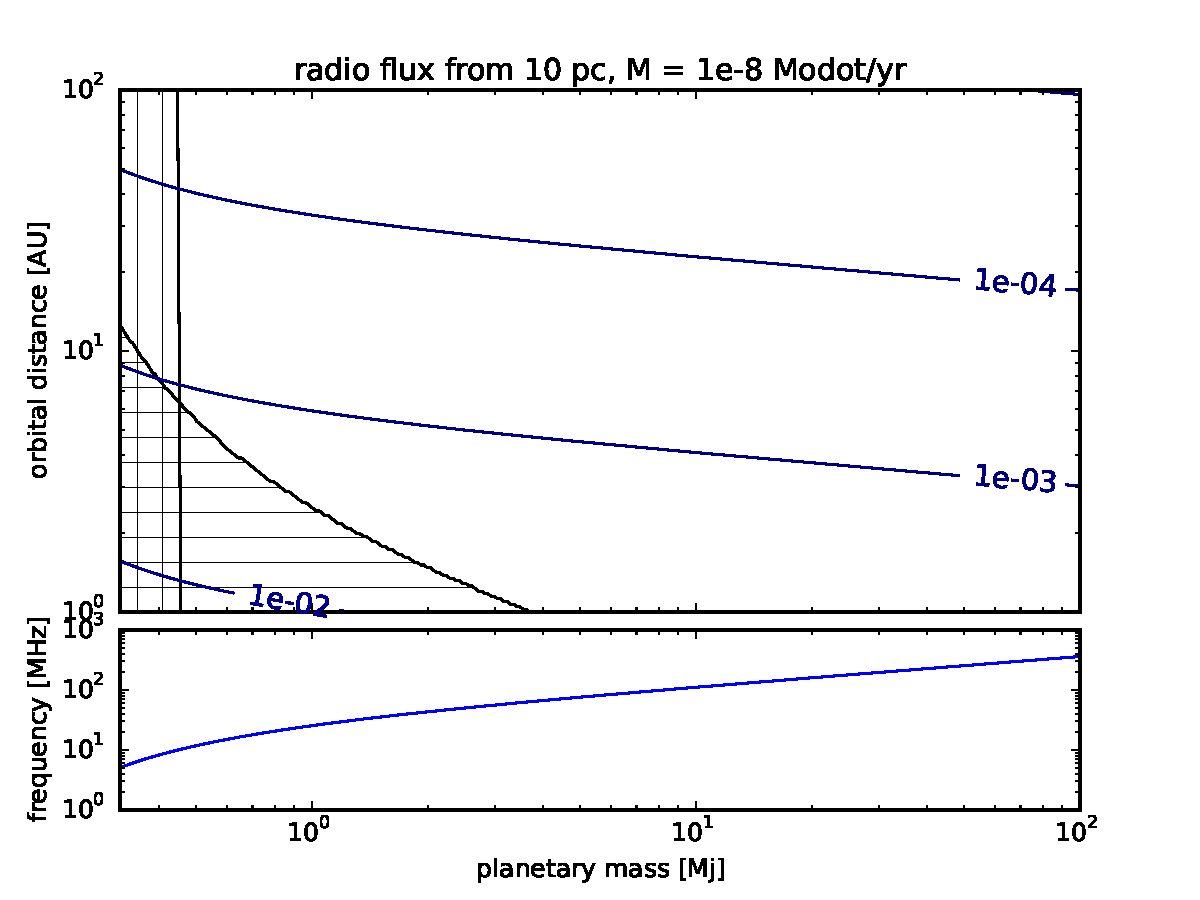
\includegraphics[width=\hsize]{radio_emission_Mdot1e-8_constRp.pdf}
%   \plotonesc{radio_emission_Mdot1e-8_constRp.eps}
  %\end{center}
 %\end{minipage}
 %\begin{minipage}{0.5\hsize}
   %\begin{center}
   %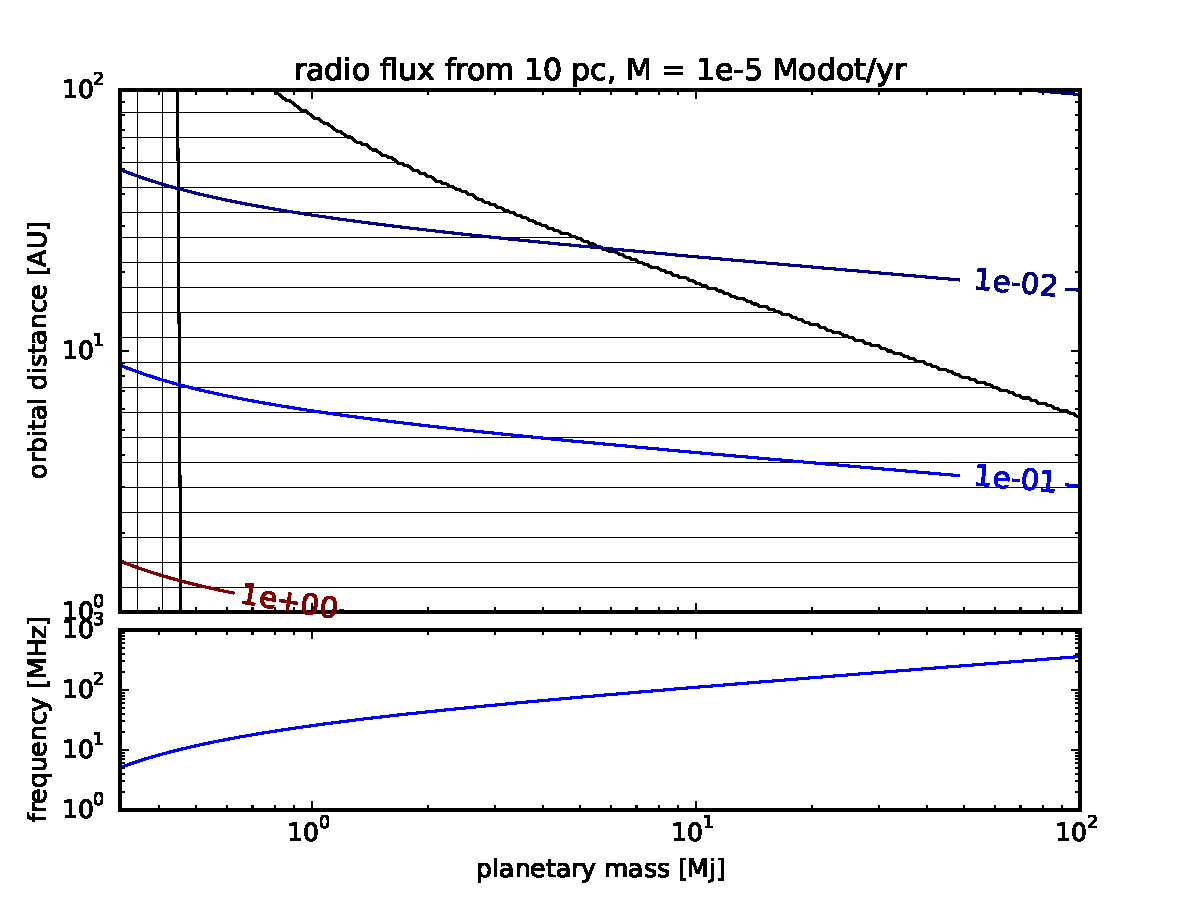
\includegraphics[width=\hsize]{radio_emission_Mdot1e-5_constRp.pdf}
%   \plotonesc{radio_emission_Mdot1e-5_constRp.eps}
  %\end{center} 
 %\end{minipage}
%   \caption{[{\bf Old version: based on scaling relationship of Sano 1993}] Top panel: Intensity of radio emission (in the unit of Jy) from a companion to a RG star (left) and an AGB star at 1 pc. The hashed region with vertical lines are not observable because of the plasma frequency cut-off of Earth's ionosphere. The hashed region with horizontal lines are not observable because of the plasma frequency cut-off of the stellar wind plasma in the vicinity of the companion. Bottom panel: cyclotron frequency, i.e., the frequency of radio emission. }
%  \label{fig:radio}
%\end{figure*}
%%%%%%%%%%%%%%%%%%%%%%%%%%%%%%%%%%%

%%%%%%%%%%%%%%%%%%%%%%%%%%%%%%%%%%%%%%%%%%%%%%%%%%%%%%%%%%%%%%%%%%%
\section{Observability}
\label{s:observability}
%%%%%%%%%%%%%%%%%%%%%%%%%%%%%%%%%%%%%%%%%%%%%%%%%%%%%%%%%%%%%%%%%%%

In this section, we discuss the observability of the estimated radio emission. 
An obvious potential obstacle is the intrinsic radio emission from host red-giant stars themselves; if they are bright relative to the radio flux from the planets, it is significantly more difficult identify the planetary contribution.
We will see in \S\ref{ss:RGradio} that radio flux from the planets will probably be larger in a certain parameter range. 
Then, we estimate the radio emission of Jupiter-twin around known M giants in \S\ref{ss:actualMgiants}. 
In \S\ref{ss:detectability}, we estimate the sensitivities and limitations of several current and future
radio instruments at relevant frequencies.
Finally, \S\ref{ss:timevariability} discusses the polarization and the expected time variability of the radio emission as means to discern the signals from the background noise. 


%%%%%%%%%%%%%%%%%%%%%%%%%%%%%%%%%%%%%%%%%%%%%%%%%%%%%%%%%%%%%%%%%%%
\subsection{Intrinsic radio emission of red giants stars}
\label{ss:RGradio}
%%%%%%%%%%%%%%%%%%%%%%%%%%%%%%%%%%%%%%%%%%%%%%%%%%%%%%%%%%%%%%%%%%%

Over the last four decades there have been numerous radio continuum observations of nearby red giants, many with the aim of understanding the extended atmospheres and mass-loss mechanisms of K- and M-type giants~\citep[e.g.,][]{Newell1982, Knapp1995, Skinner1997, Lim1998, OGorman2013}.
Almost all observations have been carried out 
%at wavelengths of 6 cm and below, 
at frequencies $\geq 5~\rm GHz$, 
probing thermal Bremsstrahlung emission from the large, partially ionized envelopes surrounding the giant stars~\citep{drake1986}.
The spectral index of this emission is of order unity, with a range of reported values for various sources between 0.8 and 1.6~\citep{OGorman2013}.

Only two published studies describe attempts to detect continuum emission from single (non-binary) red giant stars 
%at wavelengths above 20 cm 
at frequencies below 1 GHz ($L$ band); both yielded null results.
First, a program that observed a sample of nine M-type giants at 430 MHz with the Arecibo Telescope failed to detect any of the sources down to flux density 10 mJy~\citep{Fix1976}.
Later, with the Molonglo Observatory Synthesis Telescope (MOST), a sample of eight K- and M-type giants were observed at 843 MHz; the upper limits of their flux densities were placed at approximately 1 mJy~\citep{Beasley1992}.
Current facilities could achieve far deeper sensitivity on similar targets.
For example, as listed in Table~\ref{tab:sens}, the Giant Metrewave Radio Telescope (GMRT) at 150 MHz reaches a sensitivity better than 0.5~mJy in under an hour.
However, any re-attempts to detect single red giants at wavelengths near 1 meter remain to be presented in the literature.

The only red giants that have been detected at meter wavelengths are those in interacting binary systems like those of the RS CVn type.
For example, van den Oord and de Bruyn detected plasma maser emission from II Pegasi at 360 MHz and 609 MHz with the WSRT~\citep{vandenOord1994}.
Although single dwarf-type main sequence stars are also known to exhibit bright, coherent radio flares~\citep{Bastian1990}, no analog to this non-thermal emission process has been proposed to exist for evolved stars.

Altogether, we lack firm observational constraints on the brightnesses of M giants near %1-m wavelengths.
30-300 MHz frequencies. 

However, assuming thermal Bremsstrahlung emission continues to dominate in this wavelength regime, we can extrapolate down from the reported centimeter flux densities, using the specific spectral index. 
%In this case, for example, extrapolating from the 0.4 mJy flux density of $\alpha$ Ori at 1.46 GHz, and using its spectral index 1.32~\citep{Newell1982}, we arrive at an estimated flux density of 0.04 mJy at 300 MHz. 
% YF: This is consistent with the following equation, so I removed it to avoid redundancy. 
%
For example, \citet{OGorman2013} reported $\alpha$~Boo ($R_\star = 25.4 R_{\odot }$, $T=4286$ K, $d=11.26$ pc) at 1~GHz is about 70 $\mu$Jy, and $\alpha$~Tau ($R_\star = 44.2  R_{\odot }$, $T=3910$ K, $d=20.0$ pc) at 3~GHz is about 40 $\mu$Jy. 
Using these data, we extrapolate the radio flux from the host star $F_{\star}$ to the lower frequency range with a simple power law as follows:
%%%
\begin{eqnarray}
\nonumber F_{\star}(\nu ) &\sim & (0.4-1.4) \times 10^{-5} ~\mbox{Jy} \times \\
&& \left( \frac{d}{100 ~\mbox{pc}} \right)^{-2} \!\! \left( \frac{R_{\star }}{100~R_{\odot}} \right)^2 \!\! \left( \frac{\nu}{1~\mbox{GHz}} \right)^{\alpha_* } 
\end{eqnarray}
%%%
where the power index $\alpha_* $ is order of unity. 

Figure \ref{fig:cartoon} is a cartoon for a radio spectrum of a planet with $10~M_J$ and that of the host red giant star with 100~$R_{\odot }$, both of which are placed at a distance of 100 pc. 
Note that the thermal contribution from the accretion disk is negligible in this figure. \memoYF{check} 
The spectral shape is modeled by simply scaling the Jovian radio spectrum (e.g. Figure 8 of \cite{zarka_et_al2004}). 
The continuum lines from the star in the cases of $\alpha_* =0.8$ and $2.0$ are shown as an extreme case. %; the 0.6 value is the prediction from the constant property wind model \citep{wright1975,panagia1975,olnon1975}. 
As Figure \ref{fig:cartoon} indicates, with a reasonable range of spectral index, the radio emission from the star is smaller by order of magnitude than the expected radio flux from RGHJs at frequencies below 300~MHz. 
For less massive planets (with weaker magnetic fields), the distinction is even clearer, as the peak flux is larger and the peak frequencies are smaller. 


Therefore, in the following, we ignore the radio emission from the red giant as a noise source. 


%%%%%%%%%%%%%%%%%%%%%%%%%%%%%%%%%%%
\begin{figure*}[tbp]
   \plotonesc{cartoon_10Mj_100pc_smooth.pdf}
   \caption{A cartoon of radio emission spectra of a RGHJ with 10$M_J$ and the host red giants with 100 $R_{\odot }$.
The spectrum of RGHJ is modeled after Jovian radio spectra, e.g. figure 8 of \citet{zarka_et_al2004} and figure 2 of \citet{griesmeier2007a}; contribution from Io is not shown here.
The spectra of the host red giant are modeled simply by extrapolating observed radio spectra above 1~GHz with power law. }
  \label{fig:cartoon}
\end{figure*}
%%%%%%%%%%%%%%%%%%%%%%%%%%%%%%%%%%% 



%%%%%%%%%%%%%%%%%%%%%%%%%%%%%%%%%%%%%%%%%%%%%%%%%%%%%%%%%%%%%%%%%%%
\subsection{Radio Flux from Nearby M giants}
\label{ss:actualMgiants}
%%%%%%%%%%%%%%%%%%%%%%%%%%%%%%%%%%%%%%%%%%%%%%%%%%%%%%%%%%%%%%%%%%%

%%%%%%%%%%%%%%%%%%%%%%%%%%%%%%%%%%%
\begin{figure}[tbhp]
   \plotoneh{radio_1Mp.pdf}
   \plotoneh{radio_10Mp.pdf}
%   \plotoneh{radio_1Mp_5AU.pdf}
%   \plotoneh{radio_5Mp_5AU.pdf}
%   \plotoneh{radio_2Mp_4-5Gyr.pdf}
%   \plotoneh{radio_4Mp_4-5Gyr.pdf}   
   \caption{Radio emission from existing M-type red giants with a hypothetical planetary companion of 1$M_J$ and 10$M_J$ at 1 AU and 5AU.
Cross symbols indicate that the radio emission is not observable because cyclotron frequency is less than plasma density around the planet. }
  \label{fig:observability}
\end{figure}
%%%%%%%%%%%%%%%%%%%%%%%%%%%%%%%%%%% 

In order to examine the potential to detect radio emission of RGHJs with the current and near-future instruments, we estimate the possible radio emission from known red giants assuming that they have planetary companions. 
For this purpose, we obtained the list of M-type red giants from Table 4 of \citet{dumm1998} with the data of mass, radius, and effective temperature.
For each red giant, the mass-loss rate is estimated by the improved Reimers' equation \citep{reimers1975} given by \citet{schroder2005,schroder2007}:
%%%
\begin{equation}
%\dot M_\star [M_\odot{\rm /yr}] \sim 4 \times 10^{-13} \eta \left( \frac{R_{\star }}{R_{\odot }} \right)\left( \frac{L_{\star }}{L_{\odot }} \right) \left( \frac{M_\star}{M_\odot} \right)^{-1}
\dot M_\star [M_\odot{\rm /yr}] \sim 8 \times 10^{-14} \frac{\tilde L \tilde R}{\tilde M} \left( \frac{T_{\rm eff}}{4000} \right)^{3.5} \left( 1 + \frac{g_{\odot }}{4300 g_{\star}} \right) \label{eq:mass-loss}
\end{equation}
%%%
where $\tilde L = L_{\star }/L_{\odot }(=4\pi R_{\star }^2 T_{\star }^4)$, $\tilde R = R_{\star }/R_{\odot }$, $\tilde M = M_{\star }/M_{\odot }$, and $g$ is the surface gravity. 
The velocity of the stellar wind is assumed to scale with the escape velocity, hence
%%%
\begin{equation}
v \propto \sqrt{\frac{2GM_\star}{R_{\star }}}
\end{equation}
%%%
The age of the system is assumed to be roughly the same as the lifetime of the main-sequence stage, which depends on the stellar mass. We simply assume:
%%%
\begin{equation}
t \sim 10\,{\rm Gyr}\, \left( \frac{M_{\star}}{M_{\odot }} \right)^{-2.5}
\end{equation}
%%%
In addition, the distance to the system is obtained based on the parallax data from Hipparcos datasets.\footnote{http://www.rssd.esa.int/index.php?project=HIPPARCOS}

Using these data, we can now calculate the maximum frequency and intensity of radio emission by specifying planetary mass and orbital distance of a hypothetical planetary companion. 
We consider [A] a Jupiter-twin whose cyclotron frequency is $\sim 30$~MHz, and [B] a larger Jovian planet with $M_p\sim 10M_p$ whose cyclotron frequency is $\sim 300$~MHz (equations (\ref{eq:scalingB}) and (\ref{eq:fcyc})). 

Figure \ref{fig:observability} displays the estimated radio intensity (i.e., cyclotron frequency) of Jupiters [A] and [B] around M-type red giants within 100~pc. 
Jupiters are placed at 1 AU and at 5 AU for reference. 
The difference of the symbols indicates whether the radio emission can escape from the system (circle) or not (cross). 
For a hypothetical Jupiter-mass planet at 5 AU, a reasonable number of systems have potential to emit radio wave at the level of $\sim 10 \mu {\rm Jy}$  out to $\sim 100-150$ pc. 

%\memoYF{Up to where would the planet be engulfed by evolved stars? References?}
%I wondered this because if planets at 1 AU would be engulfed anyway it would not be worth discussing here. According to e.g. Nordhaus and Spiegel (2013) it is the case--however, some planets may migrate inward within 1 AU after evolution. So it should be ok. In any case this is not the main point of this paper and I would leave it out. 


%%%%%%%%%%%%%%%%%%%%%%%%%%%%%%%%%%%%%%%%%%%%%%%%%%%%%%%%%%%%%%%%%%%
\subsection{Luminosity function of planetary radio: 
nearby faint object v.s. far luminous object}
\label{ss:Lfunc}
%%%%%%%%%%%%%%%%%%%%%%%%%%%%%%%%%%%%%%%%%%%%%%%%%%%%%%%%%%%%%%%%%%%

In principle, if the expected luminosity function and positional distribution of possible RGHJ emitters were known, one could estimate the likelihood of detecting RGHJs in radio surveys. 
For illustration we consider a hypothetical power-law distribution for the RGHJ luminosity function $N[L] \propto L^{-\alpha_L}$, where, $N[L]$ is the number of objects per unit volume with a luminosity of $L$, and assume an isotropic distribution of sources in the observed volume. 
Under these assumptions, the largest luminosity in a volume limited sample (volume $V$) would be such that $V n[L] = 1$, i.e., $L \propto d^{3/\alpha _L}$.
The flux of such target at distance $d$ is $F \propto d^{\frac{3}{\alpha_L} - 2}$. 
Therefore,the likelihood of finding the brighter source increases with distance for $\alpha_L < 3/2$. 
Such a scenario would indeed be favorable to detect RGHJs given that RGs and AGB stars with high mass loss rates are rare and would require probing out to larger distances for detection. 
For example, for an $N[L] \propto L^{-1}$ the apparently brightest source within a given distance will increase linearly with distance, making it favorable for detecting intrinsically rare objects. 
Therefore, if we can estimate the luminosity function of RGHJ emitters, we may estimate their detectability.

Planning future targeted surveys of RGHJs would require accurate distribution functions of various parameters of giant stars in our neighborhood of the Galaxy.
In order to estimate the true luminosity function of RGHJ emitters, one of the key factors is the distribution of mass-loss rates of giant host stars. 
As discussed in Section~3.2,\memoDS{Replace ``3.2'' with the section label.} for a given set of orbital parameters the luminosity ($L$) of a RGHJ depends on the stellar mass-loss rate and wind velocity as $\dot{M}_\star^{2/3} v^{5/3}$. 
Employing equation (\ref{eq:mass-loss}) which implies $\dot{M}_\star \propto L_\star^{7.5/4} R_\star^{-0.75} M_\star^{-1} (1+A/g_\star)$ and crudely estimating the wind velocity as $v \propto \sqrt{GM/R} \propto M^{1/2} R^{-1/2}$, the luminosity of the RGHJ radio emission is given by $L \propto L_\star^{2/3} R_\star ^{-1/6} M_\star^{1/6} T_{\rm eff}^{2.3} (1+A/g_\star)^{2/3}$. 
Given that the dependences on $R_\star$ and $M_\star^{1/6}$ are relatively weak and that $T_{\rm eff}$ does not change significantly, the radio luminosity of RGHJs scales roughly as $L \propto L_{\star }^{2/3}$.
Thus, the criterion $\alpha_L < 3/2$ is satisfied if the slope of the luminosity function of the host stars is shallower than $-1$.



%%%%%%%%%%%%%%%%%%%%%%%%%%%%%%%%%%%%%%%%%%%%%%%%%%%%%%%%%%%%%%%%%%%
\subsection{Detectability with Current and Near Future Low Frequency Radio Instrumentation}
\label{ss:detectability}
%%%%%%%%%%%%%%%%%%%%%%%%%%%%%%%%%%%%%%%%%%%%%%%%%%%%%%%%%%%%%%%%%%%

%%%%%%%%%%%%%%%%%%%%%%%%%%%%%%%%%%%%%%%%%%%%%%%%%%%%%%%%%%%%%%%%
\begin{deluxetable*}{cccccc}
\tabletypesize{\footnotesize}
\tablecolumns{6}
\tablecaption{Detectability of Hot Jupiters with Current 
and Future Radio Telescopes.\label{tab:sens}}
\tablehead{
Instrument & Band  & \sigRMS\tablenotemark{a} & $\tau$\tablenotemark{b}  & Resolution & $\sigma_c$\tablenotemark{c}\\
           & (MHz) & ($\mu$Jy~hr$^{1/2}$)         &  (hr)                    & (\arcsec)  & ($\mu$Jy bm$^{-1}$)} 
\startdata
LOFAR-LBA  &  30-80  & 700   & 120000             & 8.3  & 42 \\ 
LOFAR-HBA  & 110-200 &  35   &    310             & 3.3  & 1.1 \\  
HERA       &  30-80  & 870   & 160000             & 1030 & 4.2$\times10^5$\\ 
GMRT       & 130-190 & 430   &  46000             & 16.5 & 56.9 \\ 
%LWA       &  30-80  & 58000 &  702127141         & 10.3 & 42.2 \\
%MWA       &  30-80  & 29000 &  176223211         & 1030 & 4.2$\times10^5$ \\
SKA-Low (part) & 50-200 & 7.8 &  12.6             & 7.6  & 9.7 \\
SKA-Low (full) & 50-350 & 2.2 &  1.0              & 4.8  & 1.5 \\
%VLA 4-Band& 30-80   & 3300  & 2312058            & 28.6 & 330 \\
VLA-LOBO   &  50-350 &  92   &  1800              & 8.6  & 10.4
\enddata
%\tablecomments{Time estimates to reach 2~$\mu$Jy RMS.}
\tablenotetext{a}{RMS noise in a 1-hour observation, computed for imaging of the full band reported 
in this table (Equation~\ref{eq:rms_sens}).}
\tablenotetext{b}{The integration time in hours required to reach an RMS of 2~$\mu$Jy (i.e.\ 5-$\sigma$ detection
of a typical source at 100~pc with 10~$\mu$Jy bm$^{-1}$ average flux).}
\tablenotetext{c}{Source confusion RMS contribution.}
\end{deluxetable*}
%
% HERA
% http://reionization.org/wp-content/uploads/2015/05/HERA0_imaging.pdf
%
% LOFAR
% https://www.astron.nl/~heald/test/sens.php; 
% 24 core stations, 16 remote, 8 international, 488 subbands
%
% GMRT
% http://gmrt.ncra.tifr.res.in/~astrosupp/obs_setup/sensitivity.html
%
%%%%%%%%%%%%%%%%%%%%%%%%%%%%%%%%%%%%%%%%%%%%%%%%%%%%%%%%%%%%%%%%

We consider in this section several current and near future radio observatories that operate at frequencies $\nu \lesssim 350~\rm MHz$ and can reach continuum sensitivities less than 1~mJy in a few hours.
The results are summarized in Table~\ref{tab:sens}. 

The primary limitation to detectability is a telescope's sensitivity, characterized by the root mean square (RMS) noise fluctuations in the sky and receiver.
The RMS noise \sigRMS\ in an interferometric observation with integration time $\tau$, bandwidth $\Delta \nu$, effective area $A_{\rm eff}$ ($\approx0.7 \pi (D/2)^2$ for interferometers comprising antennas with dish size $D$), and $N$ antennas is \citep[see e.g.][]{condon+ransom2016}
%%%
\begin{equation}
\sigRMS = \frac{2 k \Tsys}{A_{\rm eff} \, \sqrt{\Delta \nu \, \tau N (N-1)}} 
\left(\frac{\rm 10^{26} Jy}{\rm W m^{-2} Hz^{-1}}\right).
\label{eq:rms_sens}
\end{equation}
%%%
Here, \Tsys\ is the blackbody temperature equivalent of the total system noise, which is the sum of the instrument or receiver noise temperature \Trx\ and the noise contribution from the sky \Tsky.
We estimate \Tsky\ using the low frequency sky noise temperature fit from \cite{Rogers+Bowman2008}:
%%%
\begin{equation}
\Tsky = T_{150} \left( \frac{\nu}{150~\rm MHz}\right)^{-\beta} + \Tcmb
\label{eq:Tsky}
\end{equation}
%%%
where $T_{150} = 283.2~\rm K$ is the \Tsky\ at 150~MHz, $\beta=2.47$, and $\Tcmb = 2.73~\rm K$ is the contribution from the cosmic microwave background (CMB).
While this relation was fit to data taken in the 100-200~MHz range, the authors found it to be consistent with published measurements from 10-408~MHz. 
%The \Trx\ is the receiver noise temperature, which depends on the instruments and is described below. 

An additional contribution to the noise is due to source confusion, the imaging noise associated with unresolved interloping radio sources in an observation.
Source confusion is characterized by the standard deviation $\sigma_c$ in the surface brightness of an image due to one or more unresolved sources in the beam solid angle (for a review, see \cite{Condon1974,Condon2012}).
To estimate $\sigma_c$, reported in Table~\ref{tab:sens}, we use the relations provided by \cite{condon+ransom2016}, reproduced below:
%%%
\begin{eqnarray}
\sigma_c & \approx & 0.2 \left( \frac{\nu}{1 \rm~GHz} \right)^{-0.7} \left( \frac{\theta}{1\arcmin} \right)^2\!\!\!\!,~(\theta > 10\arcsec) \\
\sigma_c & \approx & 2.2 \left( \frac{\nu}{1 \rm~GHz} \right)^{-0.7} \left( \frac{\theta}{1\arcmin} \right)^{10/3}\!\!\!\!\!\!\!\!\!\!,~(\theta < 10\arcsec).
\end{eqnarray}
%%%
The source confusion limit is dominated by active galactic nuclei, which have low polarization fractions $\lesssim2.5\%$ \citep{Stil2014} and slowly vary with time.
Therefore both the circularly polarized nature of the cyclotron emission from hot jupiters and the time variability (discussed in \S\ref{ss:timevariability}) partially mitigate the source confusion limit, allowing hot jupiters, like other time-variable sources, to be detected below the imaging confusion limit.
We therefore expect confusion not to be a strong limitation to the detectability of hot jupiters.

% LOFAR
The LOw-Frequency ARray (LOFAR) operates as two separate arrays defined by their high and low bands, differing configurations, and antenna designs, which are called respectively the Low Band Antennas (LBA) and High Band Antennas (HBA).
LOFAR-LBA operates in the 10-90~MHz range, and LOFAR-HBA operates in the 100-240~MHz range \citep{vanHaarlem2013}.
We consider it as two separate instruments here.
LOFAR-LBA's most sensitive band is centered at 60~MHz, and LOFAR-HBA's is at 150~MHz.
Given the strong frequency dependence of the effective aperture of a dipole antenna, and that the reciever noise temperature for LOFAR $\Trx \sim \Tsky$, we use the LOFAR Image Noise calculator\footnote{Heald; \url{http://www.astron.nl/~heald/test/sens.php}}, which is based on {\it SKA Memo 113}\footnote{Nijboer, Pandey-Pommier, \& de Bruyn; \url{http://www.skatelescope.org/uploaded/59513\_113\_Memo\_Nijboer.pdf}}, to obtain the sensitivity and imaging parameters in Table~\ref{tab:sens}.

% HERA
The Hydrogen Epoch of Reionization Array (HERA\footnote{\url{http://reionization.org/}}) \ldots \memoYF{write here (Aaron?)}

% GMRT
The Giant Metre-wave Radio Telescope (GMRT) is an array comprising thirty 25-meter antennas, operating at frequencies 130-2000~MHz.
The lowest band (130-190~MHz) exhibits receiver noise $T_{\rm rx}$ comparable to the sky noise.
To be conservative, we use the GMRT online calculator.\footnote{\url{http://gmrt.ncra.tifr.res.in/~astrosupp/obs\_setup/sensitivity.html}}


% SKA
The low frequency component of the Square Kilometer Array (SKA), recently rebaselined to have 0.4~km$^2$ collecting area in 130,000 elements with baselines extending to 65~km, will operate from 50-350~MHz.\footnote{\url{https://www.skatelescope.org/news/worlds-largest-radio-telescope-near-construction/}}
We estimate the noise in the lower half of the band ($\nu<200~\rm MHz$), appropriate for lower mass ($\lesssim 10 M_J$) separately from the full band, which could be used to detect $\sim 30 M_J$ hot Jupiters.
We again adopt the \cite{Rogers+Bowman2008} relation for \Tsys\ (Equation~\ref{eq:Tsky}), and assume $\Trx \approx 60~\rm K$.
We caution that these assumptions are optimistic, and the time estimates could in reality be a factor of a few worse.

% VLA
For the low frequency receivers (28-80~MHz; 4-Band) in the Very Large Array (VLA) have $\Trx \sim 260~\rm K$, similar to the receiver noise temperatures for the Long Wavelength Array (LWA) \citep{Hicks2012}.  As noted in \citep{Hicks2012}, this noise level is subdominant to \Tsky\ by at least -6~dB.
Future upgrades to the VLA such as the LOw Band Observatory \citep[LOBO][]{Kassim2015IAU} are being considered, and could potentially cover the full 30-470~MHz band.
We estimate the sensitivity of LOBO assuming the receiver noise extrapolates linearly from $\Trx \approx 60~\rm K$ (internal VLA memo) in P-Band (230-470~MHz) to $\Trx \approx 260~\rm K$ in 4-band, and consider just the 50-350~MHz portion of the full 30-470~MHz band.


The noise estimates shown in Table \ref{tab:sens}, together with Figure \ref{fig:observability}, indicate that, at the frequencies relevant for the detection of radio emission from Jupiter-size planets, current instrument sensitivities are generally too low.
On the other hand, for more massive exoplanets ($M_p\sim 10 M_J$) where the bulk of the radio emission would exist above 50~MHz, there is hope to detect radio emission from nearby systems with LOFAR-HBA or LOBO.
LOFAR-HBA has reasonable sensitivity to $M_p =10~M_J$ planets at 5 AU around the few closest systems as well as those around further stars but orbiting closer to the stars. 
More promising is the low frequency component of SKA, which will be able to detect the signal within one day from planets with $M_p \sim 10~M_J$ and orbital distances $\sim$5~AU around M stars $<$100~pc from Earth.




%%%%%%%%%%%%%%%%%%%%%%%%%%%%%%%%%%%%%%%%%%%%%%%%%%%%%%%%%%%%%%%%%%%
\subsection{Discriminating the Signal from the Background}
\label{ss:timevariability}
%%%%%%%%%%%%%%%%%%%%%%%%%%%%%%%%%%%%%%%%%%%%%%%%%%%%%%%%%%%%%%%%%%%


Since the confusion limit is on the same order as the signal (Table \ref{tab:sens}), it is crucial to consider the ways to discriminate the signal from these sources. In this section, we discuss time variability and polarization as keys to identify the auroral radio emission from the planets. 

One of the key features that makes planetary radio emission distinct is the nearly  complete circular polarization \citep[e.g.][and reference therein]{dessler1983}. 
On the other hand, active galactic nuclei, which are the major confusion sources, are known to have low polarization fractions $\lesssim2.5\%$ \citep{Stil2014}. 

Another key is the significant time variability of the planetary radio emission. 
The factors that influence time variability are listed below. 

\paragraph{Modulation due to planetary spin rotation (a few hours $\sim $)}
The probability of the occurrence of the Jovian radio burst is correlated with the spin rotation phase \citep{dessler1983} due to the misalignment between the magnetic axis and the spin axis. If the time resolution of the observations is high enough, we might detect the periodicity due to planetary spin rotation. 
%
\paragraph{Modulation due to the presence of satellites (a few days $\sim $)}
The occurrence probability of Jovian radio burst is affected by the location of Io as well \citep{dessler1983}, because Io disturbs the surrounding electromagnetic field. 
Likewise, if the exoplanets have moons that emit plasmas, then the radio flux is  modulated by the orbital motion of the moon \citep[see e.g.,][]{noyola2014}. 

\paragraph{Variability of stellar wind (a few months $\sim $)?}
If the stellar wind passing the planet is variable, any modulation of the plasma density would also lead to time variabililty of planetary radio emission.  Such variability might be expected to occur on timescales of several months to half-a-year as many M giants have semi-regular periodicities on the order of a few hundred days \citep{Kiss:1999aa}.

%
\paragraph{Modulation due to orbital motion of the planet (a few years $\sim $)}
If the planetary orbit is close to the edge-on configuration, the radio emission disappears synchronously to the orbital period, due to the increased plasma cut-off frequency along the path and/or secondary eclipse.
The former is because when the planet is behind the star the path of the radio emission toward the Earth comes through the vicinity of the star where the plasma density is high.
The probability of the latter one, secondary eclipse, is $\sim a/R_\star \sim 9$\% (in the case that $a=5~\mathrm{AU}$ and $R_{\star}=100R_{\odot }$). 
%



%%%%%%%%%%%%%%%%%%%%%%%%%%%%%%%%%%%%%%%%%%%%%%%%%%%%%%%%%%%%%%%%%%%
\section{Discussion}
\label{s:discussion}
%%%%%%%%%%%%%%%%%%%%%%%%%%%%%%%%%%%%%%%%%%%%%%%%%%%%%%%%%%%%%%%%%%%


%%%%%%%%%%%%%%%%%%%%%%%%%%%%%%%%%%%%%%%%%%%%%%%%%%%%%%%%%%%%%%%%%%%
\subsection{Implication for discovery and characterization of exoplanets}
\label{ss:implication}
%%%%%%%%%%%%%%%%%%%%%%%%%%%%%%%%%%%%%%%%%%%%%%%%%%%%%%%%%%%%%%%%%%%


So far, more than 60 exoplanets are found around evolved stars \citep[e.g.][and references therein]{trifonov2015}. 
Therefore, one possible strategy is to target known planetary systems.  
One complication of the radial velocity observations of evolved stars is the high degree of jitter due to chromospheric activities and stellar pulsations, which typically produces RV errors of $\sim 30$ [m/s]. 
Therefore, there are some parameter spaces where current radial velocity observations have not been able to survey. For this parameter space, radio emission would work as a  probe to discover the possible sub-stellar companions. 

%For now, it is difficult to detect planetary-mass companions around low-mass evolved stars through other means. 
%The major difficulty in radial velocity measurement is the stellar pulsation (rms of $>30m/s$ for K giants). If the orbital period is long enough compared to the period of pulsation, it is possible to average out the pulsation and detect radial velocity of planetary component, but this requires long period monitoring. For transit observation Pulsation also contributes to the noise in detecting transit signals \memoYF{?} and besides the transit signals would be as low as 1ppm. Due to the great luminosity of the host star, direct imaging is also difficult \memoYF{?}. Thus, for the time being, one would have to aim at discovering planetary companions around evolved stars, rather than targeting at known planetary systems. 

Once radio emission is detected, it provides some useful information through both time dependence and frequency dependence. 
As mentioned in \S\ref{ss:timevariability}, auroral radio flux significantly varies in time in association with several physical processes. In turn, we could utilize the time variability to characterize the system. For example, if the time resolution of the observation is sufficiently high (with full SKA, for instance), the time variation associated with planetary spin rotation could also be detectable. 
Long term monitoring could reveal the time variability corresponding to orbital period if the system is near edge-on. Modulation on timescale of a few days may imply presence of satellites. 

If the spectra are obtained, the upper cut-off frequency of the radio spectra will imply us the magnetic field strengths of the planetary surface. Such information would be most useful if we could obtain constraints on planetary mass via e.g. radial velocity observations, because once both magnetic field strength and the planetary mass is constrained, the proposed scaling law of planetary dynamo may be contested. On the other hand, the lower cut-off frequency indicates the plasma frequency in the vicinity of the planets, which might be used as a probe of the density of the stellar wind at the planetary orbit. 


%%%%%%%%%%%%%%%%%%%%%%%%%%%%%%%%%%%%%%%%%%%%%%%%%%%%%%%%%%%%%%%%%%%
\subsection{Back-reaction of a plasma flowing into a magnetic field}
\label{ss:offset}
%%%%%%%%%%%%%%%%%%%%%%%%%%%%%%%%%%%%%%%%%%%%%%%%%%%%%%%%%%%%%%%%%%%

One might expect that plasma flowing into a region permeated by a magnetic field would, by spiraling around the field lines, generate an opposing magnetic field that partially cancels the intrinsic planetary magnetic field. 
To estimate the strength of this effect, consider a uniform flow of particles of charge $e$, mass $m$, and velocity $v$ into a region of magnetic field $B$, spiraling along the initial magnetic field. 
A single charged particle moving perpendicular to the magnetic field moves in a circular orbit of radius 
%%%
\begin{equation}
r=\frac{mv_\bot }{eB}.
\end{equation}
%%%
which creates a magnetic dipole
%%%
\begin{equation}
\mu = \frac{e}{2\pi r/v_\bot} \pi r^2 = \frac{1}{2} e r v_\bot = \frac{mv_\bot^2}{2B}.
\end{equation}
%%%
The volume integral of the canceling magnetic field $B_c$ generated by a single dipole $\mu$ is
%%%
\begin{equation}
\int d^3{\boldsymbol r} B_c = \frac{8\pi}{3} \mu.
\end{equation}
%%%

Hence, for a number density $n$ of these charged particles, the fraction of canceling field to the background magnetic field is
%%%
\begin{equation}
\frac{B_c}{B} = \frac{n(mv_\bot^2/2)}{3 B^2/8\pi} < \frac{\rho_K}{3\rho_B},
\end{equation}
%%%
where $\rho_K$ and $\rho_B$ are the kinetic energy density and the magnetic energy density, respectively. 
%If the initial velocity is not perpendicular to the magnetic field, $v$ must everywhere be replaced by its perpendicular component.

Just inside the stand-off point, 
%%%
\begin{equation}
m_p n[r_{\rm mag}] v^2 < \frac{B[r_{\rm mag}]^2}{2\pi }
\end{equation}
%%%
and thus $\rho_K/\rho _B < 1$. 
When the particle spirals into the planet, 
the magnetic pressures increases (by beaming?) by 
%%%
\begin{equation}
\frac{B^2}{8\pi } \propto \frac{1}{r^6}
\end{equation}
%%%
On the other hand, the kinetic energy of the moment increases
%%%
\begin{equation}
\frac{mv^2}{2} \propto \frac{1}{r}
%\rho _K \propto \frac{1}{r}
\end{equation}
%%%
Therefore, unless the density increases more drastically than $1/r^5$, the ratio $B_c/B$ is significantly less than unity. 

%It is interesting to note that, for a plasma of protons and electrons in a stellar wind, the canceling field is clearly dominated by the contribution of protons, though the cyclotron emission is dominated by electrons. 


%%%%%%%%%%%%%%%%%%%%%%%%%%%%%%%%%%%%%%%%%%%%%%%%%%%%%%%%%%%%%%%%%%%%%%%%
\section{Conclusions}
\label{s:conc}
%%%%%%%%%%%%%%%%%%%%%%%%%%%%%%%%%%%%%%%%%%%%%%%%%%%%%%%%%%%%%%%%%%%%%%%%

In this paper, we estimate the radio brightness of distant ``hot Jupiters'' around evolved stars (RGHJ) on the assumption of the simple empirical correlation between planetary radio emission and the input kinetic energy from the stellar wind. 
Unlike the previous paper, we consider that X-ray from the accretion disk around the planetary companion ionizes the stellar wind in the vicinity of planets, which would otherwise be fairly neutral. 
Based on such a picture, the massive stellar wind of a red giant or AGB star would interact with the planetary magnetic field and input kinetic energy into the magnetosphere of a RGHJ. 
We found that the intrinsic brightness of radio emission from RGHJs are supposedly comparable to canonical hot Jupiters in close-in orbits around main-sequence stars. 

A major obstacle to observe this radio emission is the plasma cut-off frequency of the (ionized) stellar wind. Due to great density of the stellar wind, the cut-off frequency is as high as $\sim 12$ MHz for typical red giants and $\sim$ 400 MHz for typical AGB stars. 
The promising targets are massive planetary ($M_p \gtrsim 5M_J$) companions with magnetic field stronger than Jupiter (i.e., higher cyclotron frequency). 

The radio flux from a system with an exoplanet at 5 AU at a distance of 100 pc would be typically on the order of $\sim 10 \mu $Jy. 
Such signals would be detectable with SKA within a day or so. 
For a few nearby systems, or for systems with exoplanets in closer orbit, LOFAR-HBA  would also work with a reasonable integration time. 
In both cases, it is critical to consider polarization and/or time variability of planetary radio flux, in order to separate it from confused sources in the same resolution element. 

The radio intensity of the RGHJs are intrinsically $>100$ times brighter than the main-sequence counterparts. This indicates that they can be observed 10 times further away, or in 1000 times larger volume. 
This can compensate the rareness of the evolved stars at least partly. Thus, RGHJs will be reasonable targets for future search for radio lighthouse from planetary systems. 

Radio emission can be follow-up observations of known RGHJs or may also be used as probe to discover them, given the lowered sensitivity of  radial velocity methods in detecting planetary companions. 
Once the planetary radio emission is detected, it will provide a unique approach to  planetary spin, magnetic field, and presence of satellite, and potentially stellar wind properties. 


%Admittedly, uncertainties exist in the relation between radio emission of Jovian planets and the input energy from stellar wind, as well as in the scaling of planetary magnetic field. 
%Alternatively, once we detect both the gravitational perturbation and radio emission of Jovian planets, these models will be contested.
%The viability of these scaling relations will be examined in the future. 

%The planetary magnetic moment is computed based on the simple scaling relationship given by \citep{christensen2010}. 
%-about detectability
%-number of evolved stars within 100pc $\sim 1000$. 

\vspace{0.5in}

\acknowledgements

{\sc Acknowledgments}

YF is supported from the Grant-in-Aid No. 25887024 by the Japan Society for the Promotion of Science.
DSS gratefully acknowledges support from a fellowship from the AMIAS group. JN acknowledges support from NASA grant HST AR-12146.04-A and NSF grant AST-1102738.
We thank David Hogg for encouraging us to pursue calculations of exoplanetary radio emission.
NM acknowledges support from [???]. 
YF greatly acknowledges insightful and helpful discussions with Tomoki Kimura and Hiroki Harakawa. 
The portion of this research for which TM is responsible was performed under a National Research 
Council Research Associateship Award at the Naval Research Laboratory (NRL).
Basic research in radio astronomy at NRL is supported by 6.1 Base funding.


\bibliography{biblio.bib}


\newpage

\appendix



\section{Ionization Cascade}
\label{sec:AppendixB}

For an electron-hydrogen ionizing collision, we estimate the differential cross section $\sigma$ as a function of recoil energy $d\sigma / dE_{\rm recoil}$.
We approximate the bound electron as a free one at rest and use the differential cross section for scattering of two electrons (Bhabha scattering) in the non-relativistic limit:
\begin{equation}
\label{eq:dsig/dOmeg} \frac{d\sigma}{d\Omega_{\rm CM}} \sim \frac{\alpha^2}{m_e^2 v_{\rm rel}^2 \sin^4 \theta} \, ,
\end{equation}
where $\alpha$ is the fine structure constant, $v_{\rm rel}$ is the relative velocity, $\theta$ is the scattering angle in the center of mass (CM) frame, and $m_e$ is the electron mass.
The recoil energy (that is, the energy transferred to the electron at rest) is related to the scattering angle via
\begin{equation}
  \label{eq:Erec} = \frac{1}{4} m_e v_{\rm rel}^2 \left( 1 - \cos \theta \right) \, ,
\end{equation}
and hence
\begin{equation}
  \label{eq:dErec/dOmeg} \frac{dE_{\rm recoil}}{d\Omega_{\rm CM}} = -\frac{1}{4} m_e v_{\rm rel}^2 \, .
\end{equation}
We therefore have
\begin{equation}
  \label{eq:dsig/dErec} \frac{d\sigma}{dE_{\rm recoil}} \sim \frac{\alpha^2}{m_e v_{\rm rel}^2 E_{\rm recoil}^2} \, ,
\end{equation}
which is largest for small recoil energies.
Of course, $E_{\rm recoil}$ must be larger than $E_{\rm Rydberg}$ for this approximation to be meaningful.
%This suggests that if the energetic electron ends up ionizing other atoms, it is more likely to put them right at the threshold of 




\section{Comparison with previous work}
\label{sec:AppendixA}

There is a rather wide range in estimates of the radio emission from Jovian exoplanets and it is worth noting how the different models yield different answers. 

A common part is the scaling relationship between the planetary magnetic field strength and the input kinetic energy.
From equations \ref{eq:Pinp_kin} and \ref{eq:n}, the input kinetic energy scales as
%%%
\begin{equation}
P_{\rm inp,k}=nv^3 r_{\rm mag}^2 \propto \dot M_{\star} v^2 a^{-2} r_{\rm mag}^2.
\end{equation}
%%%
Combining the above equation with the scaling between the radius of the magnetic stand-off point, $r_{\rm mag}$, and the planetary magnetic field $B$ (equation (\ref{eq:stand-off-radius})), i.e.\
%%%
\begin{equation}
r_{\rm mag} \propto B^{1/3} a^{1/3} \dot M_{\star }^{-1/6} v^{-1/6}, 
\end{equation}
%%%
and assuming a constant stellar wind, we obtain:
%%%
\begin{equation}
P_{\rm inp, k} \propto B^{2/3} a^{-4/3} \dot M_{\star }^{2/3} v^{5/3}.
\end{equation}
%%%


%equation (\ref{eq:stand-off-radius})
%%%
%\begin{equation}
%r_{\rm mag} = 11.3 \, R_J \left( \frac{B}{10~\mbox{G}} \right)^{1/3}  \left( \frac{a}{5\mbox{AU}} \right)^{1/3} \left( \frac{\dot M_\star}{10^6 \dot M_\odot} \right)^{-1/6}  \left( \frac{\dot v}{10^{-1}v_{\odot }} \right)^{-1/6}
%\end{equation}
%%%
Aside from this common part, the differences originate mainly from:
\renewcommand{\theenumi}{\roman{enumi}}
%%%
\begin{enumerate}
\item Assumptions for the scaling law of radio power in terms of input energy. 
\item Assumptions for the scaling law of planetary magnetic field strength. 
\item Different normalization (assumptions for Jovian radio emission). 
\item Assumptions for band width (either $\nu_{\rm cyc}$ or $0.5\nu_{\rm cyc}$). 
\item Modeling of stellar wind
\end{enumerate}
%%%

As for i., ii. and iii., the scaling laws are summarized in Table \ref{tab:comp}. 

%%%%%%%%%%%%%%%%%%%%%%%%%%%%%%%%
\begin{table*}[htp]
\caption{Comparison for assumed scaling relationships.}
\begin{center}
\begin{tabular}{c|l|llcc} \hline \hline
%
& Paper & Radio power & Magnetic moment  & norm [W] & band width \\\hline
%
\#1 & \citet{farrell1999} & $P_{\rm radio} \propto P_{\rm sw}^{0.88} $ & $\mathcal{M} \propto \omega M_p^{5/3}$ & $4 \times 10^9$ & $ 0.5 \nu_{\rm cyc}$ \\ \hline
%
\#2 & \citet{farrell1999} & $P_{\rm radio} \propto P_{\rm sw}^{1.2} $ & $\mathcal{M} \propto \omega M_p^{5/3}$ & $4 \times 10^{11}$ & $ 0.5 \nu_{\rm cyc}$ \\
& \citet{lazio2004} & & $\mathcal{M} \propto \omega M_p^{2}$?? & & \\
& \citet{ignace2010} & & & & \\ \hline
\#3 & \citet{stevens2005} & $P_{\rm radio} \propto P_{\rm sw} $ & $\mathcal{M} \propto M_p$ & - & - \\ \hline
\#4 & \citet{griesmeier2005,griesmeier2007a,griesmeier2007b} & $P_{\rm radio} \propto P_{\rm sw}$ & $\mathcal{M} \propto \rho _c^{1/2} \omega r_c^4 $ & $2.1 \times 10^{11}$ & $ 0.5 \nu_{\rm cyc}$ \\
\#5 & & & $\mathcal{M} \propto \rho _c^{1/2} \omega^{1/2} r_c^3 \sigma ^{-1/2} $ & & \\
\#6 & & & $\mathcal{M} \propto \rho _c^{1/2} \omega^{3/4} r_c^{7/2} \sigma ^{-1/4} $ & \\
\#7 & & & $\mathcal{M} \propto \rho _c^{1/2} \omega r_c^{7/2}$ & & \\ \hline
%\#8 & \citet{griesmeier2007a,griesmeier2007b} & $P_{\rm radio} \propto P_{\rm sw}$ & same as above & $2.1 \times 10^{11}$ & $ \nu_{\rm cyc}$ \\ \hline
\#8 & \citet{reiners2010} & $P_{\rm radio} \propto P_{\rm sw}$ & $\mathcal{M} \propto M_p^{1/6} L^{1/3} R_p^{25/6}$ \\ 
 & this work & & \\ \hline
\end{tabular}
\end{center}
\label{tab:comp}
\tablecomments{}
\end{table*}
%%%%%%%%%%%%%%%%%%%%%%%%%%%%%%%%

If we use the assumptions that $R_p \sim R_J\;\;(const.)$, $\rho _c\sim R_p\sim const.$, and $\sigma = const.$, then the assumptions are reduced to:
%%%%%%%%%
\begin{eqnarray}
\mbox{[\#1]} \; P_{\rm rad} &\sim & 4 \times 10^9 \,{\rm W}\,\left( \frac{\omega}{\omega _J} \right)^{0.58} \left( \frac{M_p}{M_J} \right)^{0.98} \left( \frac{a}{a_J} \right)^{-1.17} \left( \frac{\dot M_\star}{\dot M_{\odot}} \right)^{0.586} \left( \frac{v}{v_{\odot}} \right)^{1.46} \\
%
\mbox{[\#2]} \; P_{\rm rad} &\sim & 4 \times 10^{11} \,{\rm W}\, \left( \frac{\omega}{\omega _J} \right)^{0.79} \left( \frac{M_p}{M_J} \right)^{1.33} \left( \frac{a}{a_J} \right)^{-1.60} \left( \frac{\dot M_\star}{\dot M_{\odot}} \right)^{0.8} \left( \frac{v}{v_{\odot}} \right)^{2.0} \\
%
\mbox{[\#3]} \; P_{\rm rad} &\sim & ? \times 10^{11} \,{\rm W}\,\left( \frac{M_p}{M_J} \right)^{2/3} \left( \frac{a}{a_J} \right)^{-4/3} \left( \frac{\dot M_\star}{\dot M_{\odot}} \right)^{2/3} \left( \frac{v}{v_{\odot}} \right)^{5/3} \\
%
\mbox{[\#4]} \; P_{\rm rad} &\sim & 2.1 \times 10^{11} \,{\rm W}\,\left( \frac{\omega}{\omega _J} \right)^{2/3} \left( \frac{M_p}{M_J} \right)^{1/3} \left( \frac{a}{a_J} \right)^{-4/3} \left( \frac{\dot M_\star}{\dot M_{\odot}} \right)^{2/3} \left( \frac{v}{v_{\odot}} \right)^{5/3} \, \\
%
\mbox{[\#5]} \; P_{\rm rad} &\sim & 2.1 \times 10^{11} \,{\rm W}\,\left( \frac{\omega}{\omega _J} \right)^{1/3} \left( \frac{M_p}{M_J} \right)^{1/3} \left( \frac{a}{a_J} \right)^{-4/3} \left( \frac{\dot M_\star}{\dot M_{\odot}} \right)^{2/3} \left( \frac{v}{v_{\odot}} \right)^{5/3} \, \\
%
\mbox{[\#6]} \; P_{\rm rad} &\sim & 2.1 \times 10^{11} \,{\rm W}\,\left( \frac{\omega}{\omega _J} \right)^{1/2} \left( \frac{M_p}{M_J} \right)^{1/3} \left( \frac{a}{a_J} \right)^{-4/3} \left( \frac{\dot M_\star}{\dot M_{\odot}} \right)^{2/3} \left( \frac{v}{v_{\odot}} \right)^{5/3} \, \\
%
\mbox{[\#7]} \; P_{\rm rad} &\sim & 2.1 \times 10^{11} \,{\rm W}\,\left( \frac{\omega}{\omega _J} \right)^{2/3} \left( \frac{M_p}{M_J} \right)^{1/3} \left( \frac{a}{a_J} \right)^{-4/3} \left( \frac{\dot M_\star}{\dot M_{\odot}} \right)^{2/3} \left( \frac{v}{v_{\odot}} \right)^{5/3} \, \\
%
\mbox{[\#8]} \; P_{\rm rad} &\sim & ? \times 10^{11} \,{\rm W}\, \left( \frac{M_p}{M_J} \right)^{0.69}  \left( \frac{t}{4.5 \rm~Gyr} \right)^{-0.288}  \left( \frac{a}{a_J} \right)^{-4/3} \left( \frac{\dot M_\star}{\dot M_{\odot}} \right)^{2/3} \left( \frac{v}{v_{\odot}} \right)^{5/3} \, \\
\end{eqnarray}
%%%%%%%%%
For the last equation, we used the scaling of the luminosity $L$, equation (\ref{eq:burrowsLum}):
%%%
\begin{equation}
L \sim 1.84\times10^{-10} L_\odot \left( \frac{t}{4.5 \rm~Gyr} \right)^{-1.3} \left( \frac{M_p}{M_J} \right)^{2.64} \tag{\ref{eq:burrowsLum}}
\end{equation} 
%%%
\memoYF{Note that in \citet{ignace2010} the dependence on mass-loss rate and stellar wind velocity is not taken account consistently; in that paper, $P_{\rm rad} \propto \dot M_{\star } v^2$.}

In summary, we write down the scaling of the radio emission as below, 
%%%
\begin{equation}
P_{\rm rad} \times 10^{11} \,{\rm W}\, \left( \frac{\omega}{\omega _J} \right)^{\alpha } \left( \frac{M_p}{M_J} \right)^{\beta }  \left( \frac{t}{4.5 \rm~Gyr} \right)^{-\gamma }  \left( \frac{a}{a_J} \right)^{-\delta }  \left( \frac{\dot M_\star}{\dot M_{\odot}} \right)^{\epsilon } \left( \frac{v}{v_{\odot}} \right)^{\phi } \, \\
\end{equation} 
%%%
with $\alpha = 0.5-0.8$, $\beta = 0.33-1.33$, $\gamma = 0-0.288$, $\gamma = 1.17-1.60$, $\epsilon = 0.58-0.8$, $\phi = 1.46-2.0$. 
\end{document}

\clearpage



\section{Memo}

%%%%%%%%%%%%%%%%%%%%%%%%%%%%%%%%%%%%%%%%%%%%%%%%%%%%%%%%%%%%%%%%%%%
\subsection{Brighter Implies Harder to See:\\
Greater $B$ Produces Lower $F_\nu$}
\label{ss:counterintuitive}
%%%%%%%%%%%%%%%%%%%%%%%%%%%%%%%%%%%%%%%%%%%%%%%%%%%%%%%%%%%%%%%%%%%


The cyclotron frequency at radius $r$ is:
%%%
\begin{equation}
\nu_{\rm cyc} = \frac{e B(r)}{2\pi m_e} \propto \frac{B_p}{r^3}
\end{equation}
%%
Therefore, 
%%%
\begin{equation}
\frac{dP}{d\nu_{\rm cyc}} = \frac{dP}{d\nu } \propto -\frac{r^4}{B_p} \frac{dP}{dr}
\end{equation}
%%%
Employing Larmor formula, power emitted from a thin shell at $r\sim r+dr$, $dP/dr$ is 
%%%
\begin{equation}
\frac{dP}{dr} \propto 4\pi r^2 N_{\rm plasma}(r) v_{\bot }^2(r) B^2(r) \label{eq:larmor}
\end{equation}
%%%
where $N_{\rm plasma}(r) $ represents the number density of plasma in the planetary magnetosphere at radius $r$. 

We assume that $N_{\rm plasma}(r_{\rm mag}) $  is proportional to the squared radius of the magnetic stand-off point:
%%%
\begin{equation}
N_{\rm plasma}(r_{\rm mag}) \propto \pi r_{\rm mag}^2 \;\;(\propto B_p^{2/3}) \label{eq:N0_plasma}
\end{equation}
%%%
Due the the mass flux conservation,
%%%
\begin{equation}
4 \pi r^2 N_{\rm plasma}(r) v_{\|} = const.
\end{equation}
%%%
Combining with equation (\ref{eq:N0_plasma}),
%%%
\begin{equation}
N_{\rm plasma}(r) \propto  \frac{r_{\rm mag}^2 }{v_{\|}(r) r^2} \propto  B_p^{2/3} \cdot \frac{v_{\|}(r)}{r^2}
\end{equation}
%%%

Because the magnetic dipole moment
%%%
\begin{equation}
\mu = \frac{mv_{\bot}(r)}{eB(r)}
\end{equation}
%%%
is approximately to be constant while the plasma falls down along the magnetic field, 
%%%
\begin{eqnarray}
v_{\bot }(r) \propto \frac{1}{r^3} \label{eq:v_bot} \\
B(r) \propto \frac{B_p}{r^3} 
\end{eqnarray}
%%%
On the other hand, conservation of energy ensures that
%%%
\begin{equation}
\mathcal{E} = -\frac{GM_p}{r} + \frac{v_{\bot }^2}{2} + \frac{v_{\|}^2}{2}=const.
\end{equation}
%%%
Assuming that the initial energy (at $r=r_{\rm mag}$) is negligible compared to those near the surface, $\mathcal{E}=0$, 
%%%
\begin{equation}
v_{\|}^2 \sim \frac{GM_p}{r} - \frac{v_{\bot ,0}^2}{2} \left( \frac{r}{r_{\rm mag}} \right)^{-6} \label{eq:v_||}
\end{equation}
%%%

Substituting equations (\ref{eq:N0_plasma}),  (\ref{eq:v_bot}) and (\ref{eq:v_||}) into equation (\ref{eq:larmor}) leads to
%%%
\begin{equation}
\frac{dP}{dr} \propto \frac{B_p^{8/3}}{r^{12}} \left( \frac{GM_p}{r} - \frac{v_{\bot ,0}^2}{2} \left( \frac{r}{r_{\rm mag}} \right)^{-6} \right)^{1/2}  
\end{equation}
%%%
The right-hand side has the maximum value $\sqrt{5GM_p/6\tilde r} $ at radius $\tilde r=(6v_{\bot ,0}^2/GM_p)^{1/5}$. 
At $r>>\tilde r$, 
%%%
\begin{equation}
\frac{dP}{dr} \propto \frac{B_p^{8/3}}{r^{25/2}}
\end{equation}
%%%
and
%%%
\begin{equation}
\frac{dP}{d\nu } \propto \frac{B_p^{5/3}}{r^{17/2}} \propto \frac{\nu^{17/6}}{B_p^{7/6}}
\end{equation}
%%%


At $r<<\tilde r$, 
%%%
\begin{equation}
\frac{dP}{dr} \propto \frac{B_p^{8/3}}{r^{15}}
\end{equation}
%%%
and
%%%
\begin{equation}
\frac{dP}{d\nu } \propto \frac{B_p^{5/3}}{r^{11}} \propto \frac{\nu^{11}}{B_p^{28/3}}
\end{equation}
%%%




\newpage







\memoDS{Is this section needed anymore, since this is already in the Griesmeier paper?
Does the Griesmeier paper make the point explicit enough, or is this still somewhat valuable?
Also, are we 100\% sure that this section is right?
A planet with larger surface field achieves an equivalent field to a planet with a smaller surface field at a larger radius, and captures a larger wind flux.
Should we think more about the spectrum?}





According to Eq.~(\ref{eq:Pkinp}), the total emitted power scales with $B^{2/3}$.
In detail, it is not obvious how the power spectral density scales with a planet's surface magnetic field, because the emission process involves electrons passing through a wide range of magnetic field conditions (dipolar field strength drops off as $r^{-3}$, and only in an idealized model is a planet a perfect magnetic dipole).
Nevertheless, a reasonable ansatz is that the radio emission is spread over a range of wavelengths in an approximately scale-independent way.
In other words, the frequency bandwidth $\Delta \nu$ of Eq.~(\ref{eq:Fnu}) is proportional to $\nu_{\rm cyc}$, as described in Section~\ref{ss:model_intensity} and in \citet{griesmeier2007b}.
This means that the power spectral density is likely to scale as the total power divided by the cyclotron frequency corresponding to a characteristic field strength where the emission peaks.
Since $\nu_{\rm cyc}$ scales as $B$ (a higher power of $B$ than the scaling of total power), this implies that the power spectral density in the radio scales as $B^{-1/3}$.
Planets that are intrinsically brighter, owing to a greater magnetic field strength, probably have their emission spread out over a broader set of frequencies, and therefore have a lower flux density as measured in Janskys!
\memoDS{Is this pointed out elsewhere in the literature?}



\section{Dave's sketch}

\citep{spiegel2008}

\citep{lecavelier_et_al2013}

\citep{janhunen_et_al2003}

\citep{zarka1992, zarka1998}

\citep{farrell_et_al2004}

\citep{lazio+farrell2007}: likelihood function, tau Boo search

\citep{lecavelier_et_al2009}

\citep{spiegel2012}

\citep{nordhaus+spiegel2013}



\citep{jiang+jin1996}: 12cm radio of Jupiter during Shoemake-Levy-9

\citep{morin2012, morin_et_al2013}

\citep{christensen_et_al2009, christensen2010}

\citep{saar2001}: Inverse rossby number scaling of magnetic field: $B
\sim 60 {\rm~G} \times Ro^{-1.2}$.  Here, he takes $Ro = \tau_c/P_{\rm
  rot}$, where $\tau_c$ is the convective turnover time = ?
\citep{gilliland1986}.  Well, $F \sim \rho v_c^3 \sim \rho
(H/\tau_c)^3$, so $\tau_c \sim H (\rho / F)^{1/3} = H / (\sigma T_{\rm
  eff}^4 / \rho)^{1/3}$.  Alternatively, $\tau_{\rm conv} \sim (M R^2
/ L)^{1/3}$.

On dimensional grounds, the convective turnover time goes as
$\tau_{\rm conv} \sim (M R^2 / L)^{1/3}$.  According to
\citet{burrows_et_al2001}, radius $R$ and luminosity scale with time
as $R \sim R_J$, where $R_J$ is the radius of Jupiter, and
\begin{equation}
\frac{L}{10^{-9} L_\odot} \sim \left( \frac{t}{1 \rm~Gyr} \right)^{-1.3} \left( \frac{M}{1~M_J} \right)^{2.64} \, .
\label{eq:burrowsLum_2}
\end{equation}
So,
%\begin{eqnarray}
%\nonumber \tau_{\rm conv} & \sim & 3 {\rm~days} \times \left( \frac{M}{M_J} \right)^{1/3} \left( \frac{R}{R_J} \right)^{2/3} \left( \frac{L}{L_\odot} \right)^{-1/3} \\
% & = & 
%\end{eqnarray}
\begin{eqnarray}
\nonumber \tau_c & \sim & 3 {\rm~hrs} \times \frac{\left( \frac{H}{100 \rm~km} \right) \left( \frac{\rho}{10^{-5} \rm~g~cm^{-3}} \right)^{1/3}}{\left( \frac{L}{10^{-9} L_\odot} \right)^{1/3}} \\
 & = & 3 {\rm~hrs} \times \frac{\left( \frac{H}{100 \rm~km} \right) \left( \frac{\rho}{10^{-5} \rm~g~cm^{-3}} \right)^{1/3}}{\left( \frac{M}{1 ~M_J} \right)^{0.88} \left( \frac{t}{1 \rm~Gyr} \right)^{0.43}} \\
\end{eqnarray}
So the Rossby number $Ro = \tau_c/P_{\rm rot}$ is
\begin{eqnarray}
Ro & = & \frac{\tau_c}{P_{\rm rot}} \\
 & = & \left( \frac{P_{\rm rot}}{3 \rm~hrs} \right)^{-1} \times \frac{\left( \frac{H}{100 \rm~km} \right) \left( \frac{\rho}{10^{-5} \rm~g~cm^{-3}} \right)^{1/3}}{\left( \frac{M}{1 ~M_J} \right)^{0.88} \left( \frac{t}{1 \rm~Gyr} \right)^{0.43}}
\end{eqnarray}

\citep{hallinan_et_al2013}

\citep{desch+kaiser1984} radiometric Bode's law

Noting that
\begin{equation}
\dot{M}_* = 4\pi r^2 \rho[r] v \, ,
\label{eq:mdot}
\end{equation}
so $\rho[r] = \dot{M}_*/(4\pi r^2 v)$,
\begin{eqnarray}
\frac{\rho v^2}{2} = \frac{B^2}{8\pi} \sim \frac{B_0^2}{8\pi} \left( \frac{d}{d_0} \right)^{-3} \, ,
\end{eqnarray}
where $B_0$ is the field strength at a distance $d_0$ from the planet.
\begin{eqnarray}
\frac{\rho v^2}{2} & \sim & \frac{B_0^2}{8\pi} \left( \frac{d}{d_0} \right)^{-6} \\
\frac{\dot{M}_* v}{8\pi a^2} & = & \frac{B_0^2}{8\pi} \left( \frac{d}{d_0} \right)^{-6} \\
\frac{\dot{M}_* v}{r^2} & = & B_0^2 \left( \frac{d}{d_0} \right)^{-6} \\
d^6 & = & \frac{d_0^6 B_0^2 r^2}{\dot{M}_* v} \\
d_A & = & d_0 \left( \frac{B_0^2 r^2}{\dot{M}_* v} \right)^{1/6} \\
  & \sim & 4 R_J \left( \frac{d_0}{R_J}\right) \left\{ \frac{\left( \frac{B}{10 \rm~G} \right)^2 \left( \frac{r}{5 \rm~AU} \right)^2}{\left( \frac{\dot{M}_*}{10^{-6} M_\odot/\rm yr} \right) \left( \frac{v}{20 \rm~km/s} \right)} \right\}^{1/6}
\label{eq:Chapman-Ferraro}
\end{eqnarray}
In the above, $d_A$ is the distance from the planet to the Alfven
point, where the magnetic energy density $u_B = B^2 / 8\pi$ equals the
kinetic energy density in the stellar wind $u_w = \rho v^2/2$, and
$B_0$ is the magnetic field strength at distance $d_0$.

The escape speed is
\begin{equation}
v_{\rm esc}^* = \sqrt{\frac{2 G M_*}{R_*}} \, ,
\end{equation}
so if the stellar wind speed is a factor $C$ times the escape speed, then ...

The power incident on the planet within $d_A$ is
\begin{eqnarray}
P_{\rm inc} & = & \frac{\rho v^3}{2} \times \pi d_A^2 \\
\frac{\rho v^2}{2} & \sim & \frac{B_0^2}{8\pi} \left( \frac{d}{d_0} \right)^{-6} \\
d_A^6 & = & d_0^6 \frac{B_0^2}{4\pi \rho v^2} \\
d_A^2 & = & d_0^2 \left( \frac{B_0^2}{4\pi \rho v^2}\right)^{1/3} \\
\pi d_A^2 \frac{\rho v^3}{2} & = & \frac{d_0^2}{2} \left( \frac{\pi^2 \rho^2 v^7 B_0^2}{4} \right)^{1/3} \\
P_{\rm inc} & = & d_0^2 \left( \frac{\pi^2 \rho^2 v^7 B_0^2}{32} \right)^{1/3} 
%\frac{\dot{M}_* v}{8\pi a^2} & = & \frac{B_0^2}{8\pi} \left( \frac{d}{d_0} \right)^{-6} \\
%\frac{\dot{M}_* v}{r^2} & = & B_0^2 \left( \frac{d}{d_0} \right)^{-6} \\
%d^6 & = & \frac{d_0^6 B_0^2 r^2}{\dot{M}_* v} \\
%d_A & = & d_0 \left( \frac{B_0^2 r^2}{\dot{M}_* v} \right)^{1/6} \\
%  & \sim & 4 d_0 \left\{ \frac{\left( \frac{B}{10 \rm~G} \right)^2 \left( \frac{r}{5 \rm~AU} \right)^2}{\left( \frac{\dot{M}_*}{10^{-6} M_\odot/\rm yr} \right) \left( \frac{v}{20 \rm~km/s} \right)} \right\}^{1/6}
\end{eqnarray}
Note that $\rho v = \dot{M}_*/4\pi r^2$.  Therefore,
\begin{eqnarray}
P_{\rm inc} & = & d_0^2 \left( \frac{\pi^2 \rho^2 v^7 B_0^2}{32} \right)^{1/3} \\
 & = & d_0^2 \left( \frac{\dot{M}_*^2 v^5 B_0^2}{512 r^4} \right)^{1/3} \\
 & = & \frac{d_0^2}{8} \left( \frac{\dot{M}_*^2 v^5 B_0^2}{r^4} \right)^{1/3} \\
\nonumber  & \sim & 2 \times 10^{18} {\rm~W} \left( \frac{d_0}{R_J} \right)^2 \left( \frac{\dot{M}_*}{10^{-5} M_\odot / {\rm yr}} \right)^2 \\
 & & \times \left( \frac{v}{20 \rm~km/s} \right)^5 \left( \frac{B_0}{10 \rm~G} \right)^2 \left( \frac{r}{5 \rm~AU} \right)^{-4}
\end{eqnarray}


The power incident on the planet is

%\citep{lunine_et_al1989} -- error?

% http://kiss.caltech.edu/workshops/magnetic2013/presentations/winterhalter.pdf

%ftp://ftp.iwf.oeaw.ac.at/pub/Scherf/PRE-CD%20V2/pre6/nigl.pdf

%%%%%%%%%%%%%%%%%%%%%%%%%%%%%%%%%%%%%%%%%%%%%%%%%%%%%%%%%%%%%%%%%%%
\subsection{Assumptions for Planetary Magnetic Field}
%\label{ss:magneticfield}
%%%%%%%%%%%%%%%%%%%%%%%%%%%%%%%%%%%%%%%%%%%%%%%%%%%%%%%%%%%%%%%%%%%

\memoYF{It may be better to consider Cristensen's scaling, taking account of the age. But I have not followed the theory yet.}

Theoretically, the magnetic moment of gaseous planets are expressed with the following scaling relationship \citep{griesmeier2004}:
%%%%%%%%%% 
\begin{equation}
\mathcal{M} \propto  \omega ^{\alpha } \rho_c ^{\beta } r_c^{\gamma } \sigma ^{\delta }
\end{equation}
%%%%%%%%%%
where $\omega $ is the spin angular velocity, $\rho _c$, $r_c$ and $\sigma $ are the density, the radius, and the conductivity of the ``dynamo region'' where the density is high enough for hydrogen to be metallic, respectively. 
The scaling indexes are estimated to be $\alpha \sim 1/2-1$, $\beta \sim 1/2$, $\gamma \sim 3-4$, and $\sigma \sim -1/2-0$. In this paper, we assume $\alpha =1$, $\beta =1/2$, and $r_c = 7/2$ \citep{sano1993}. \memoYF{validity?}

Unlike usual hot jupiters, RGHJs are not tidally locked to their host stars, as the stellar tidal field does not change significantly even if the star evolves into a giant.
Without no physical insights of the typical spin rate, we simply assume that of Jupiter: $\omega = 9.925$ [hr]. 
\memoYF{Would their spin rate become higher or lower??}

In order to evaluate $\rho _c $ and $r_c$, we need a model of internal structure of gaseous planets. 
First, we assume that the planetary radius is constant at $R_p = R_{p,J}$, as the numerical calculations show that the radii of gaseous planets over the range of $0.1 R_{p, J} < M_p < 10M_{p, J}$ (with core mass less than 10\%) are converged to $0.8 R_{p, J} < R_p < 1.2R_{p, J}$ in 1 Gyr \citep{fortney2007}. 
For the density profile, we assume a polytrope gas sphere with index $n=1$, which results in:
%%%%%%%%%% 
\begin{equation}
\rho [r] = \left( \frac{\pi M_p}{4 R_p^3} \right) \frac{\sin \left[ \pi \frac{r}{R_p} \right]}{\left( \pi \frac{r}{R_p} \right)}. \label{eq:rho_r_2}
\end{equation}
%%%%%%%%%%
We determine the core radius $r_c$ by assuming that the hydrogen becomes metallic when $\rho (r)$ exceeds the critical density $\rho_c=700\,\mbox{kg/m}^3$. The density of the metallic core, $\rho _c$ is obtained by averaging the density in the core. 
We assume that the conductivity $\sigma $ is the same as Jupiter \memoYF{?}. 



Equation (\ref{eq:fcyc>fplasma}) can also be rewritten as: 
%%%
\begin{eqnarray}
 \left( \frac{B}{10~\mbox{G}} \right) &>& 0.526 \left( \frac{a}{5~\mbox{AU}} \right)^{-1} \\
 && \times \left( \frac{\dot M_\star}{10^6 \dot M_{\odot}} \right)^{1/2}  \left( \frac{v}{10^{-1}v_{\odot}} \right)^{-1/2} \label{eq:Ba_limit}
\end{eqnarray}
%%%
or, 
%%%
\begin{eqnarray}
 \left( \frac{M_p}{M_{p,J}} \right) &> & 0.627 \left( \frac{a}{5~\mbox{AU}} \right)^{-0.72} \left( \frac{t}{4.5~\mbox{Gyr}} \right)^{0.31} \\
 && \times \left( \frac{\dot M_\star}{10^6 \dot M_{\odot}} \right)^{0.36}  \left( \frac{v}{10^{-1}v_{\odot}} \right)^{-0.36} \label{eq:Ma_limit}
\end{eqnarray}
%%%
In other words, given any orbital distance, there is a lower mass limit for a planet to be able to release the  radio wave out of the system. 
Substituting equation (\ref{eq:Ba_limit}) into equation (\ref{eq:F_nu_RGHJ}) leads to the maximum spectral radio flux at given orbital period:
%%%
\begin{eqnarray}
F_{\nu} &<& 1.30 \times 10^{-3}~\mbox{Jy} \left( \frac{d}{10~\mbox{pc}} \right)^{-2} \\
&& \times \left( \frac{a}{5~\mbox{AU}} \right)^{1/3}  \left( \frac{\dot M_\star}{10^6 \dot M_{\odot}} \right)^{1/2} \left( \frac{v}{10^{-1} v_{\odot}} \right)^{13/6}
\end{eqnarray}
%%%




\end{document}

